\chapter{Event Reconstruction}
\label{ch:RecoCal}

The most basic form of raw data collected is a vector of hits above threshold. The MC simulation described in chapter \ref{ch:Simulation} also outputs events in this format. However, these objects by themselves are not very useful; instead, a certain level of reconstruction is required before real physics can be studied. The first major step in this process is to apply calibration so that the hits can be translated into a set of energy depositions, consistent throughout and across both detectors. Any number of algorithms can then be applied to create new objects or search for features, including tracks, the event vertex, or particle identifiers (PIDs). This chapter describes the calibration and elements of the reconstruction chain relevant to the NC disappearance analysis.

\section{Calibration}

The purpose of calibration is to ensure a uniform detector response throughout each and across both detectors. This is done in two major steps, a relative and absolute calibration. The relative calibration accounts for threshold effects and attenuation across a single cell. It is designed to create a uniform response throughout a cell and across a single detector. The absolute calibration creates a scale factor for each detector to convert the calibrated PE scale from the relative calibration into an energy unit. This section follows the SA notes in reference \cite{ref:TNCalib}.

The relative calibration is designed to convert the PE signal output from the electronics into a calibrated unit, such that two equal signals from any two detector locations mean equal true energy deposited. This part of the calibration accounts for threshold effects and attenuation in the WLS fibers, outputting a corrected PE value, the PECorr.

Hits from through-going cosmic ray muons, or muons that enter and exit the detector without stopping, are used for the relative calibration. The WindowTrack algorithm, a fast algorithm that fits straight lines through hits \cite{ref:RecoWinTrack}, is used to produce 3D tracks from the cosmic ray events, and only those with a successful reconstruction are used. Within these events, only tricell hits are used for the calibration procedure. A tricell hit is defined as a hit in cell $i$ within a given plane that also has hits in cells $i+1$ and $i-1$. Under special circumstances (low statistics, too many dead neighboring cells) different hits are used for a particular cell. The path length of the cosmic traveling through the cell and the distance from readout are calculated for all of the selected hits in a cell. The distance from readout is labeled $W$, an alias for either X or Y, such that $W = 0$ is the center of a cell and positive values of $W$ are closer to the readout. From this information, individual histograms of the average PE/cm vs $W$ are constructed for each cell. The relative calibration procedures apply corrections to these histograms.

The first effect handled by the relative calibration is of threshold and shielding. Thresholds refer to the issue that an energy deposition may not register for a hit at all, as opposed to simply being attenuated, if there are not enough photons that reach the APD. Shielding refers to the tendency of the detector mass to alter the average signal of a minimum ionizing particle, or MIP, as a function of distance to the readout. Both of these effects would bias the set of hits used by the calibration by preferably selecting hits with greater numbers of photons, in turn underestimating the true energy deposited in the cell. To account for this, a correction factor is applied for each cell,
\beq
T = \frac{PE}{\lambda} \cdot \frac{E_{True}}{E_{MIP}}
\label{eq:CalibThreshold}
\eeq

\n where $T$ is correction factor, $PE$ is the number of simulated photons that the electronics register, $\lambda$ is the number of photons that would be seen without fluctuations, $E_{True}$ is the true energy deposited in the scintillator, and $E_{MIP}$ is the energy that would be deposited based only on the particle path length through the cell. The ratio on the left accounts for the threshold correction since $\lambda$ is only dependent on the simulated threshold level, and the ratio on the right accounts for the shielding correction since $E_{MIP}$ is only depenedent on the path length. Two dimensional histograms of the correction factor as a function of the cell number and distance from the readout are made for each detector and view, then fit with a polynomial to remove noise. These histograms are then used to correct the corresponding data and MC. Figure \ref{fig:CalibThreshold} shows examples of this correction factor used for the FD.
\begin{figure}[htb]
  \centering
  \begin{tabular}{c c}
    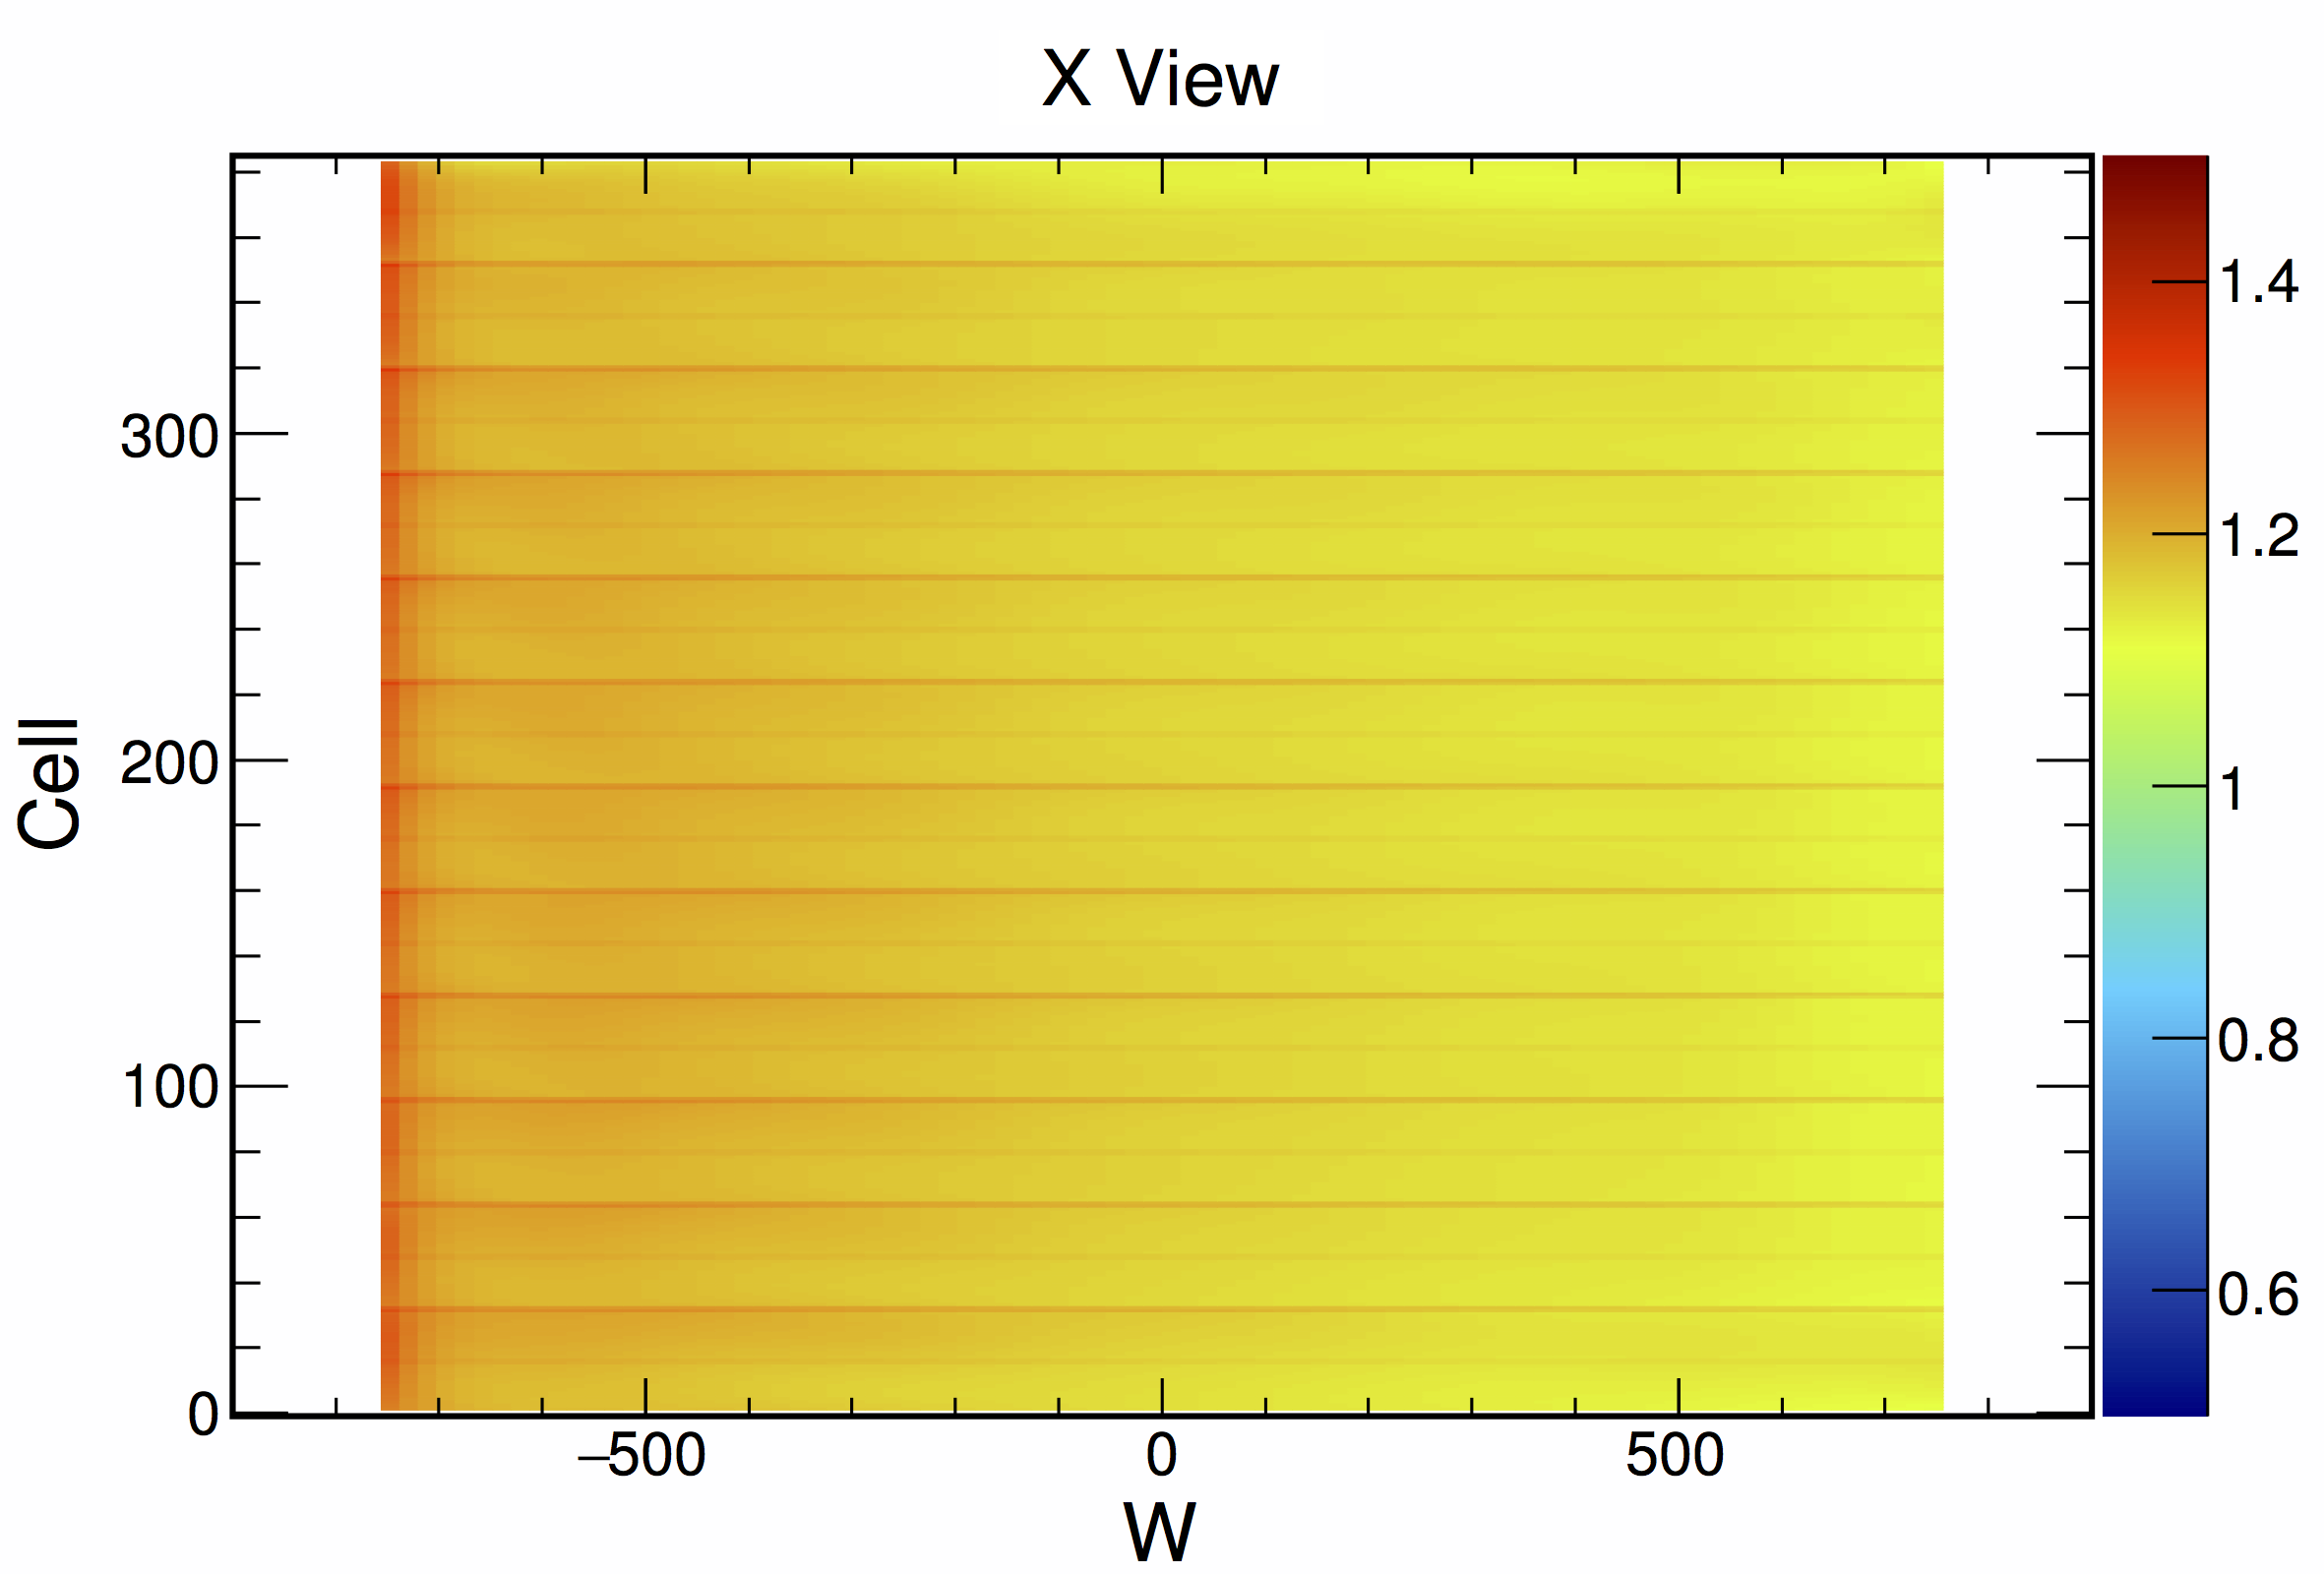
\includegraphics[width=.47\textwidth]{figures/Calib/ThresholdFDX.png} &
    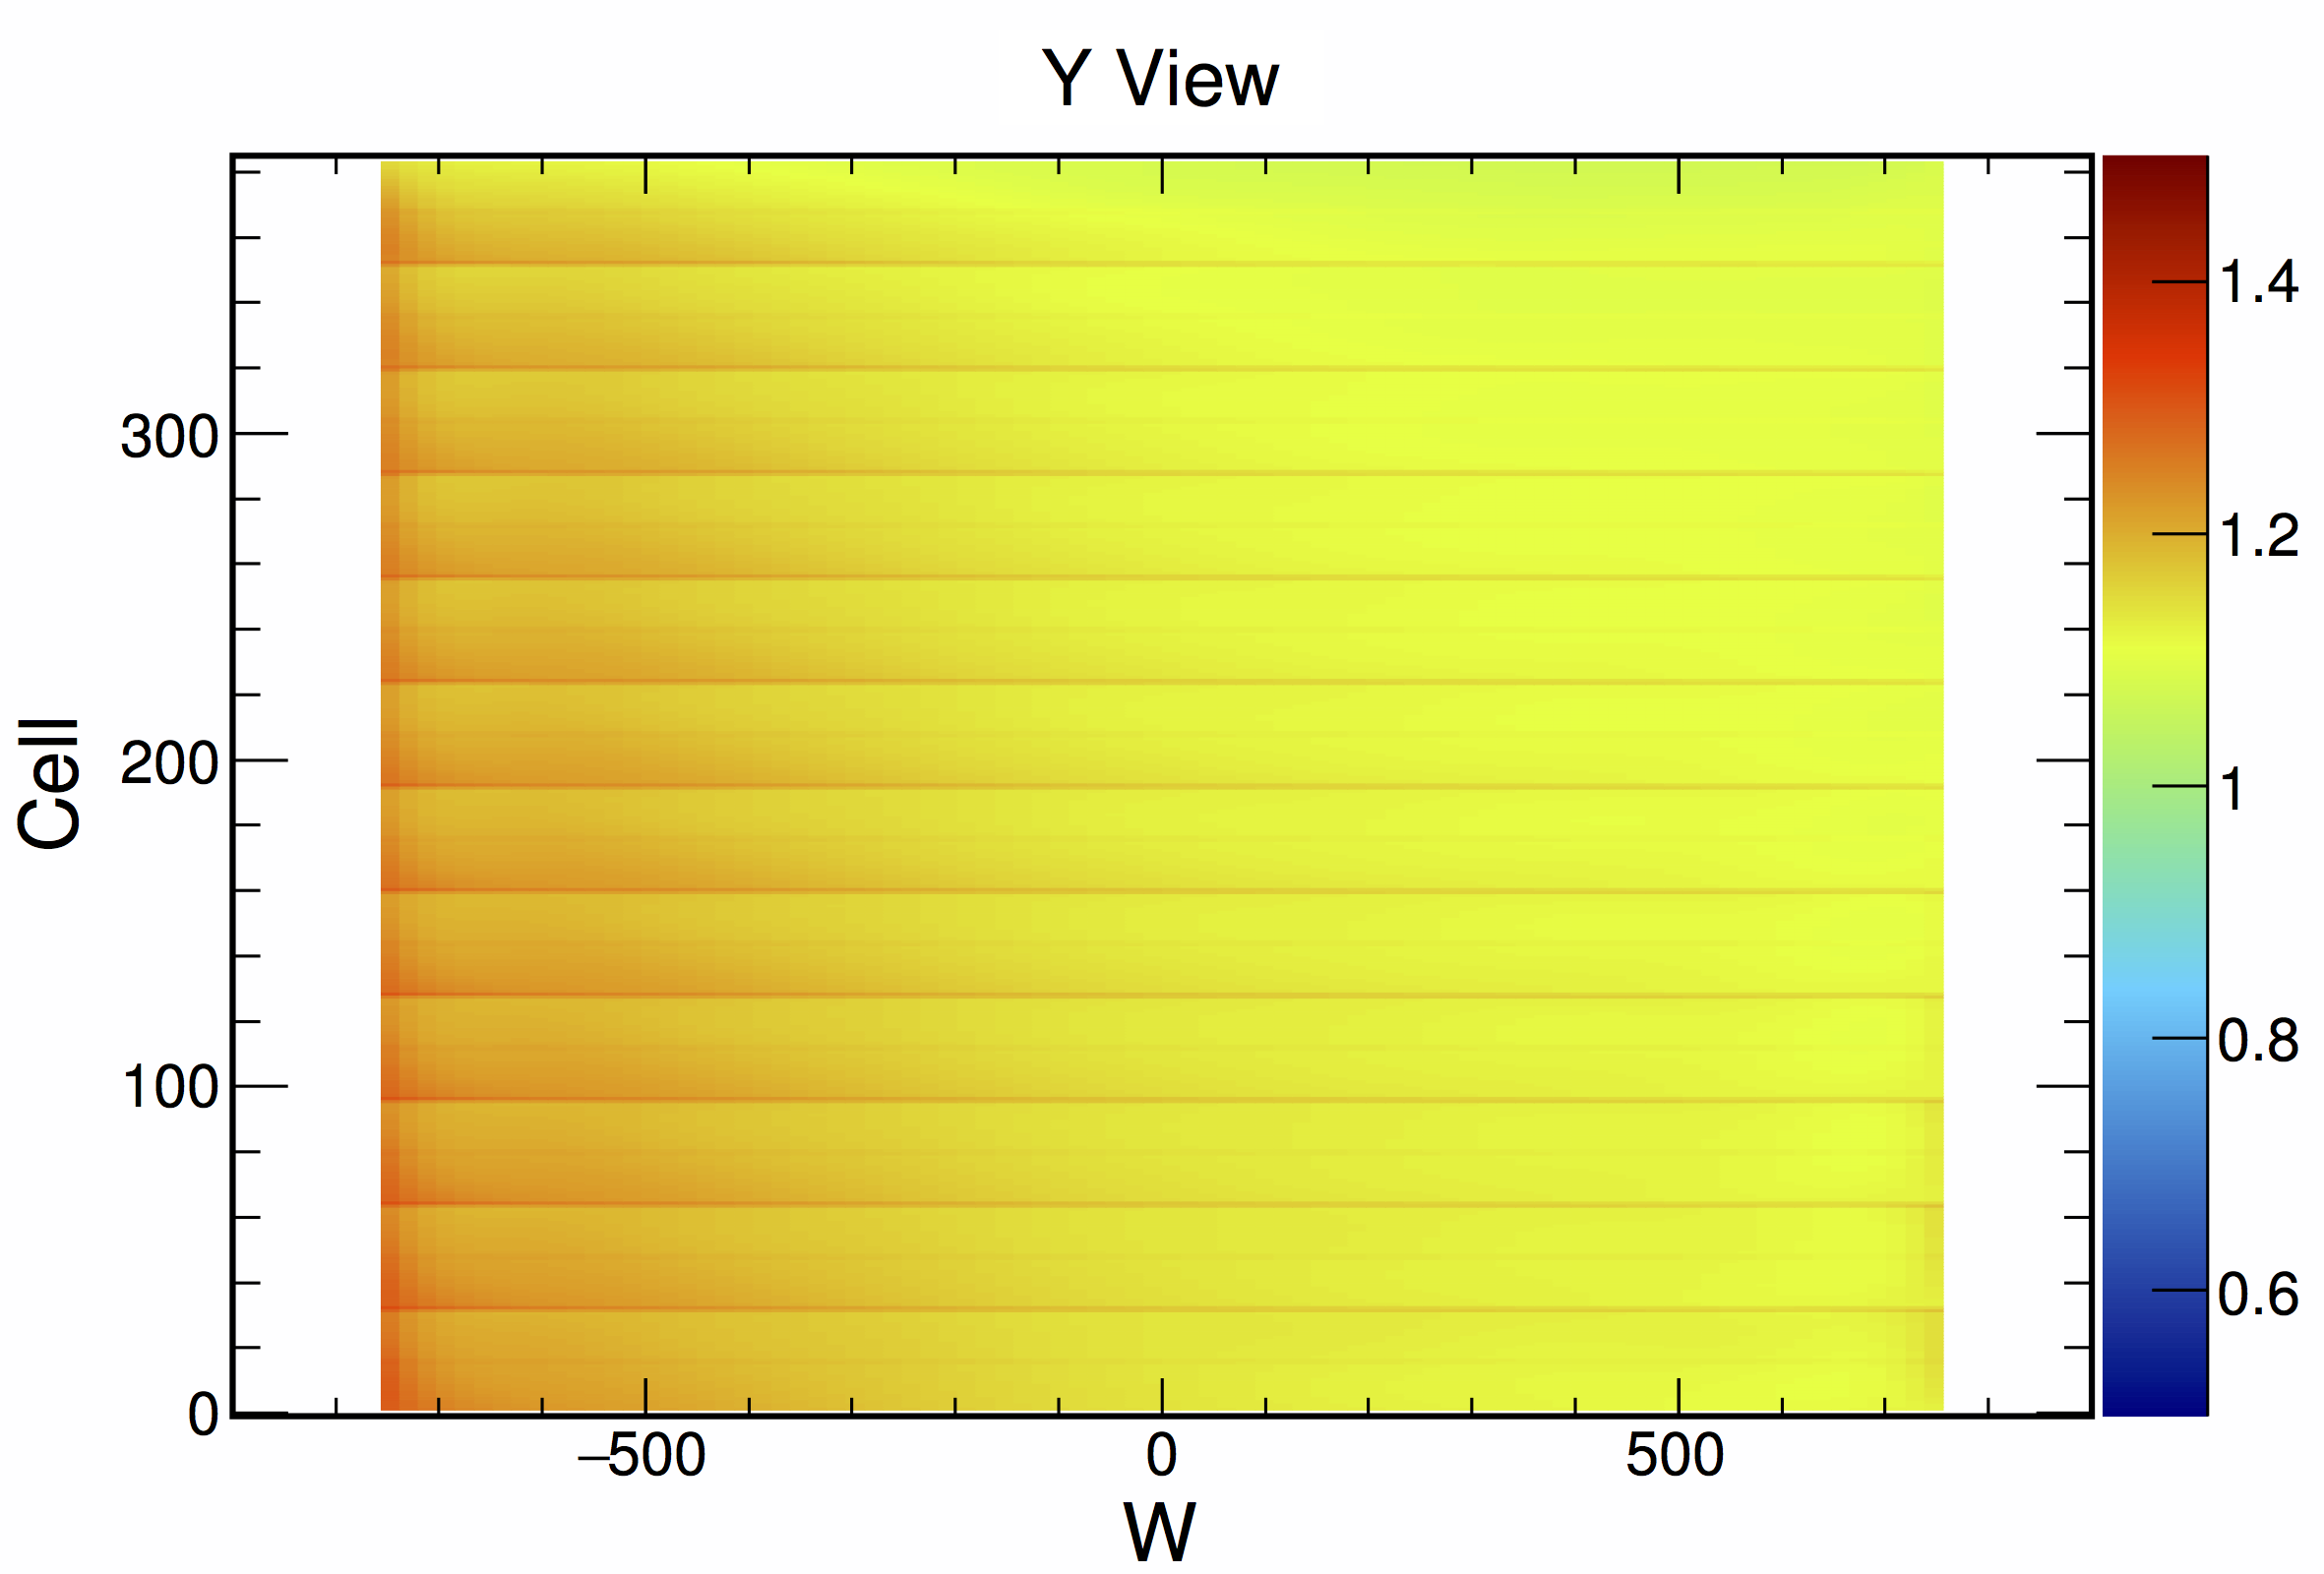
\includegraphics[width=.47\textwidth]{figures/Calib/ThresholdFDY.png} \\
  \end{tabular}
  \caption[Threshold and Shielding Correction Factors]{Correction factor for threshold and shielding effects at the FD as a function of cell number and distance from electronic readout. Cells in the X view are shown on the left, Y view on the right.}
  \label{fig:CalibThreshold}
\end{figure}

The next part of the relative calibration is the general form of the attenuation correction. Tricell hits are grouped by cell and fit to a double exponential to consider both short and long path light. For data, individual fits are performed for every single cell. In MC, a fit is performed on the group of all cells in a particular view and at the same location in a plane due to much lower simulated cosmic event statistics. The double exponential has the form
\beq
y = C + A\left(\exp\left(\frac{W}{X}\right) + \exp\left(-\frac{L+W}{X}\right)\right)
\label{eq:CalibAttenuation}
\eeq

\n where $C$, $A$, and $X$ are the free parameters, and $L$ is the full length of the cell. $X$ is the cell attenuation length. The fit excludes hits in the regions closest and furthest to the readout. It includes the range $[-750, 750]$ at the FD, $[-150, 150]$ for the fully active region of the ND and for Y view muon catcher cells, and $[-150, 50]$ for X view muon catcher cells, with all numbers in cm. These central regions are chosen to exclude the significant rolloff regions at the end of the cells, which are handled differently.

The final step in the relative calibration handles the attenuation correction at the ends of the cells and the residuals from the fit above in the central part of the cells. First, both of these regions are fit with a single LOWESS curve using a tricube weight,
\beq
w_i = \begin{cases}
\left(1 - \left| \frac{W - W_i}{\sigma} \right|^3 \right)^3 & \mbox{for } \vert W - W_i \vert < \sigma \\
0 & \mbox{for } \vert W - W_i \vert \geq \sigma \end{cases}
\label{eq:CalibRolloff}
\eeq

\n where $W$ is a local point on the curve, $W_i$ is the $i$th neighbor of the local point, $w_i$ is the weight on $W_i$, and $\sigma = 30\unit{cm}$ is the range of neighbors that affect the value of $W$. $W$ is then the weighted mean of $W_i$. Next, a simple line of the form $y = mW + c$ is fit to a collection of the neighbor points around a point, $W$, to give the corrected response, $y$. The full LOWESS curve is approximated by linear interpolation between $20$ points calculated using this procedure. The full attenuation calibration combines the results of the linear interpolation with the result of the double exponential above. Figure \ref{fig:CalibAttenuation} shows examples of the fully fit attenuation curves used in FD data calibration.
\begin{figure}[p]
  \centering
  \begin{tabular}{c c}
    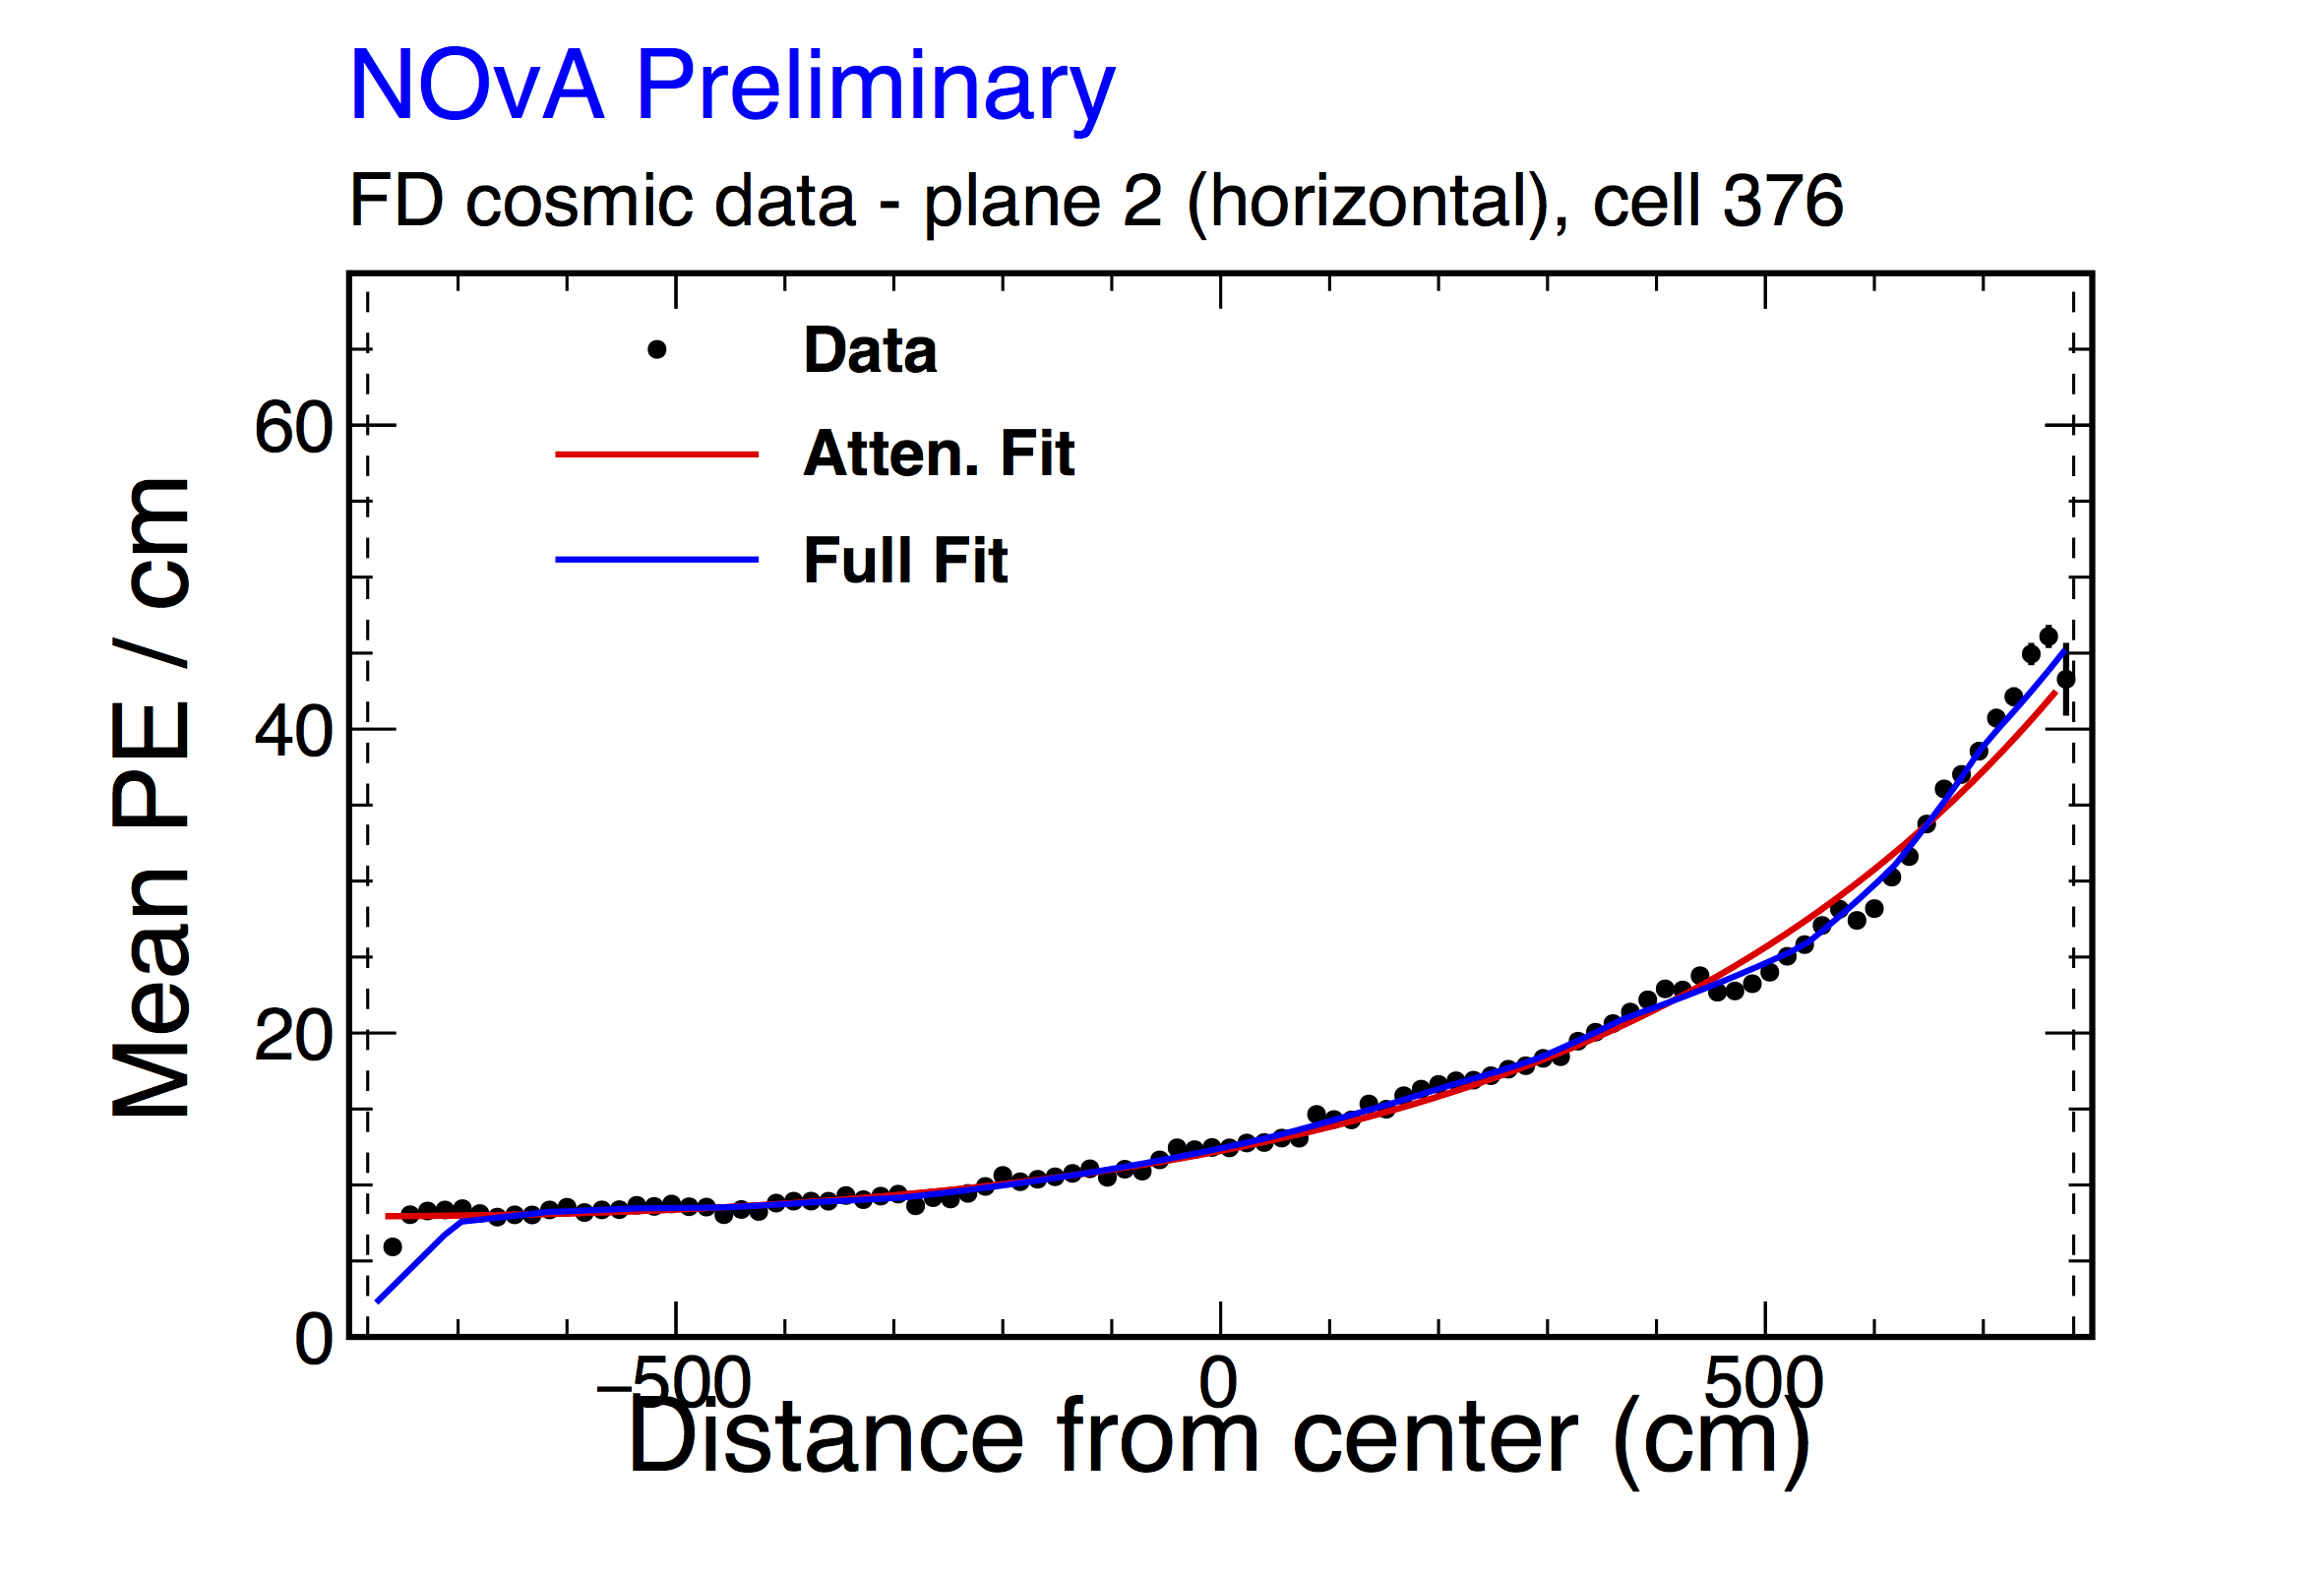
\includegraphics[width=.47\textwidth]{figures/Calib/AttenuationFDH.png} &
    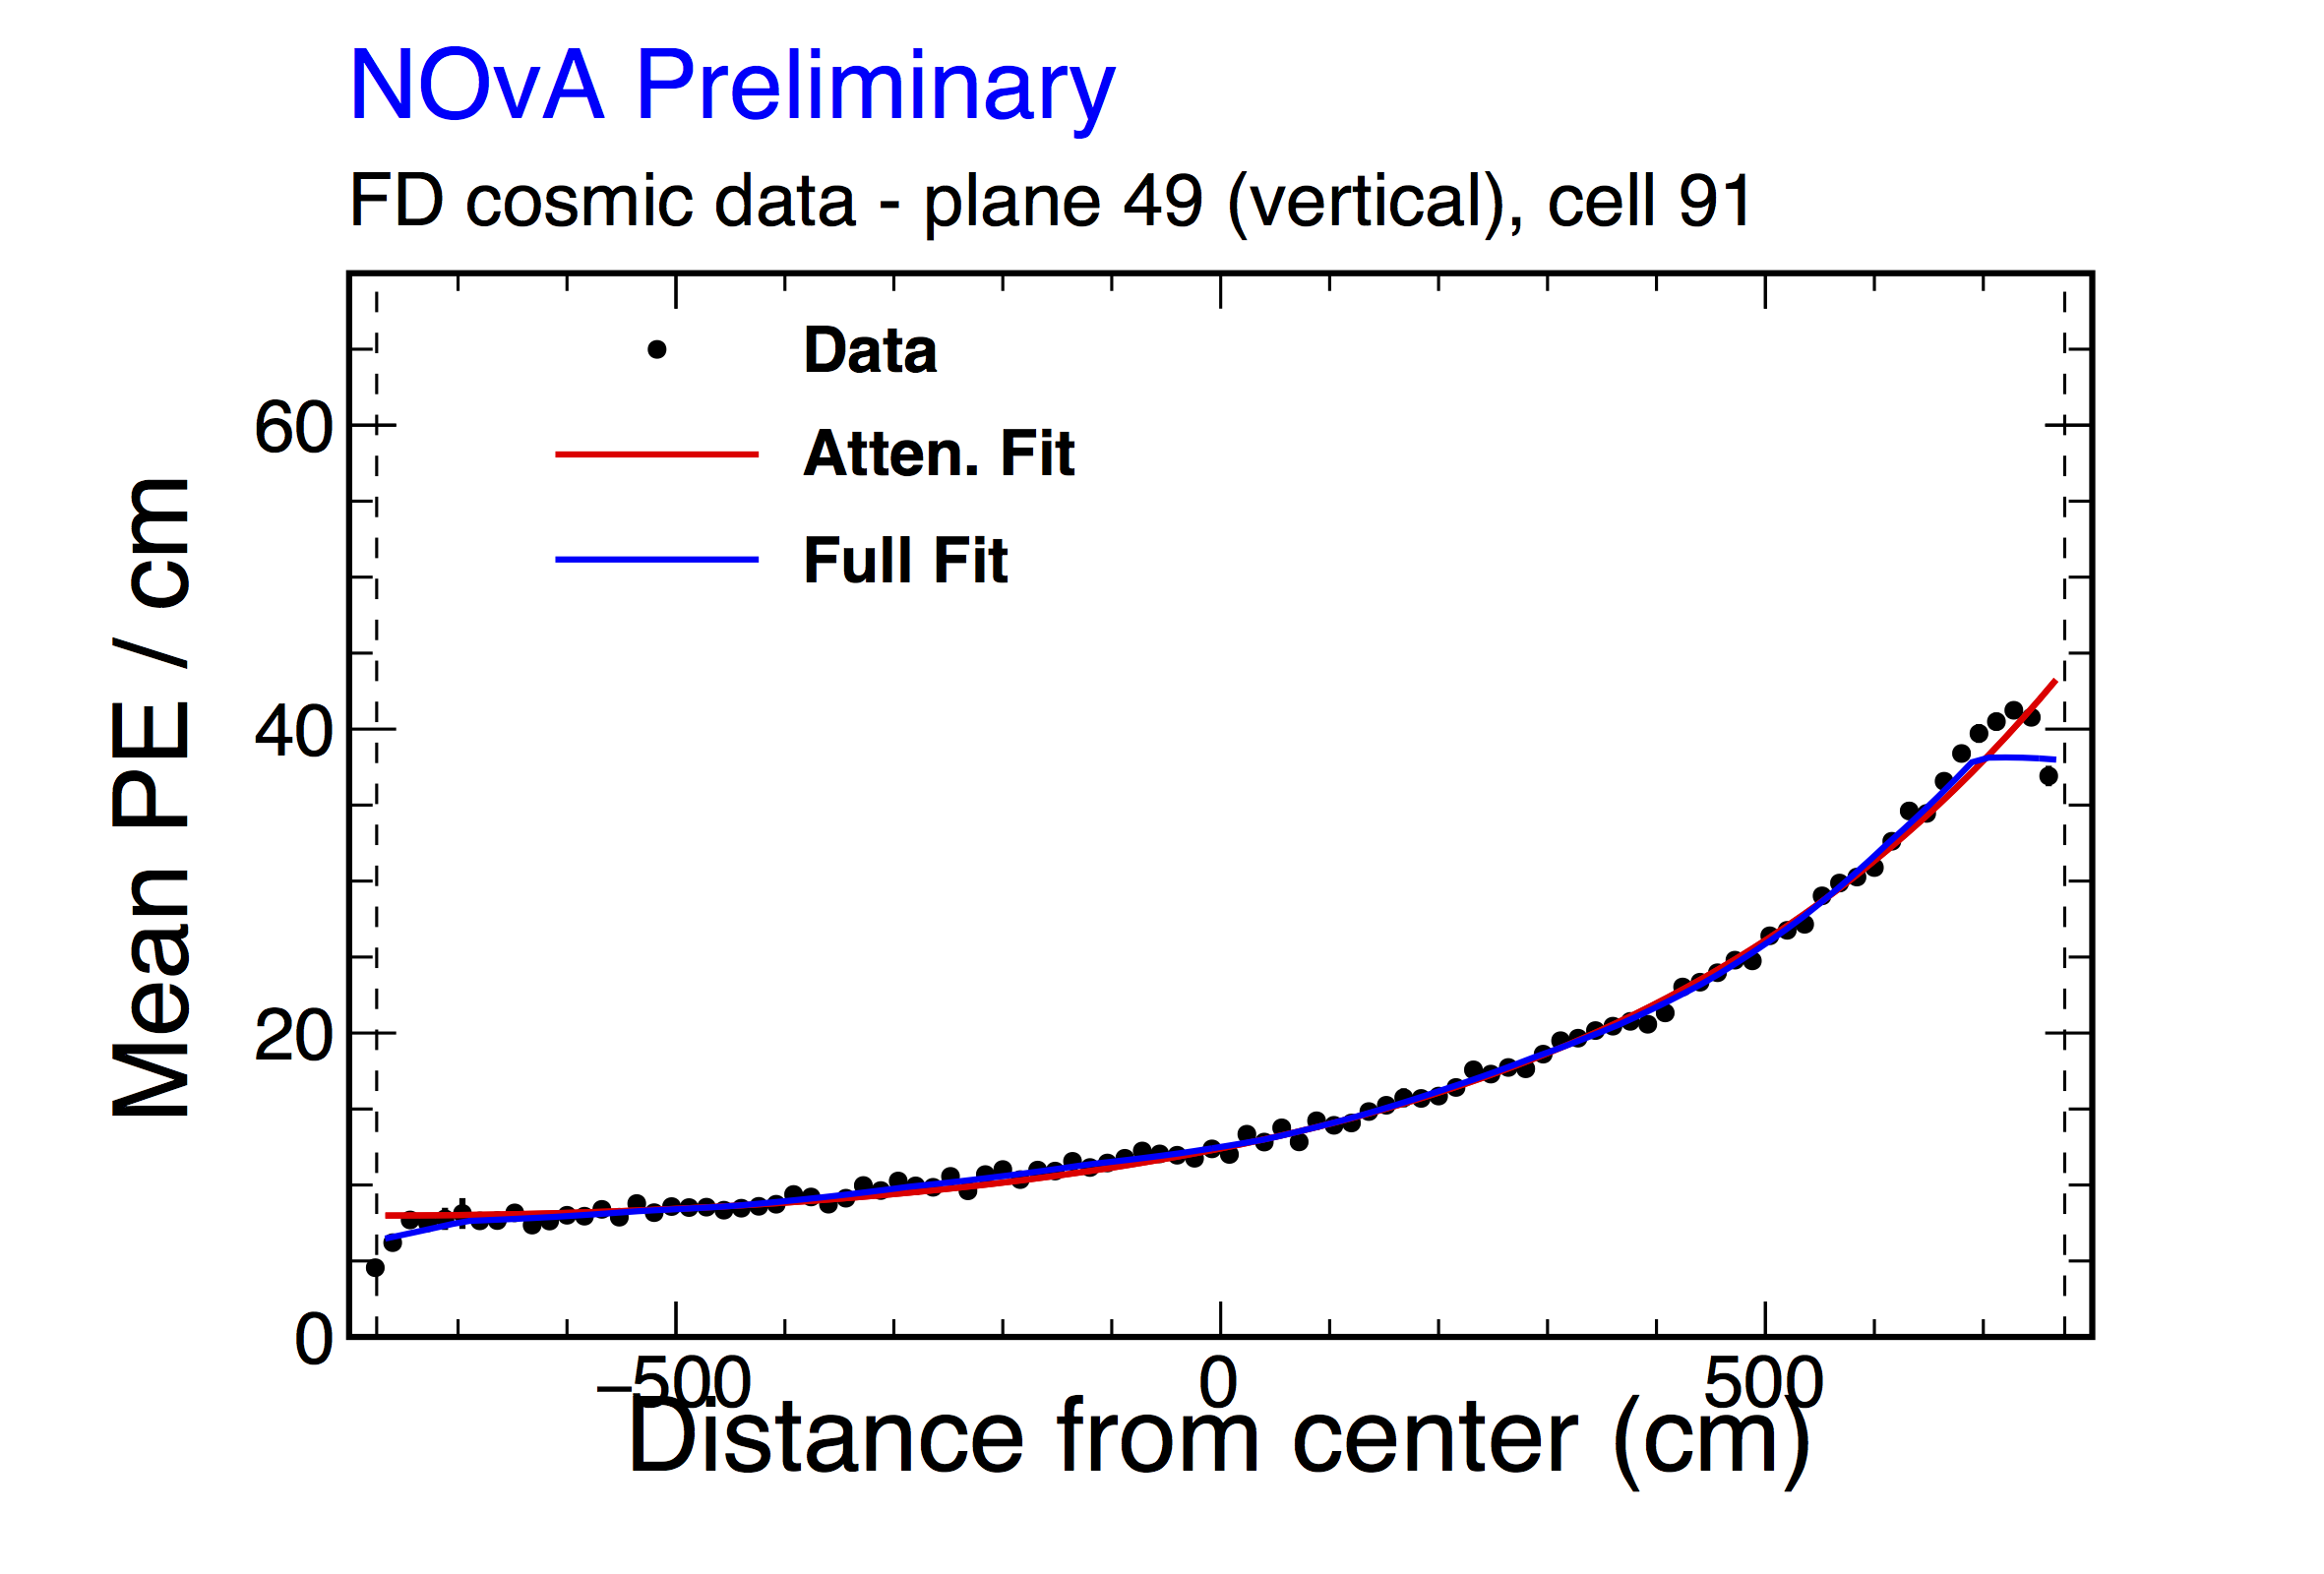
\includegraphics[width=.47\textwidth]{figures/Calib/AttenuationFDV.png} \\
  \end{tabular}
  \caption[Attenuation Fits]{Fits to the average detector response for a cell in the FD. The red curves show just the result from the double exponential fit, and the blue curves show the full fit that also includes the LOWESS correction. The left plot is an example of a horizontal view cell, the right plot is an example of a vertical view cell.}
  \label{fig:CalibAttenuation}
\end{figure}

The relative calibration combines the results of all three steps to create a uniform detector response as a function of distance to readout. Figure \ref{fig:CalibRelative} shows the MC before and after calibration is applied to assess the performance of the full procedure. The regions with deviations at the end of the cells ultimately are not used for the analysis.
\begin{figure}[p]
  \centering
  \begin{tabular}{c c}
    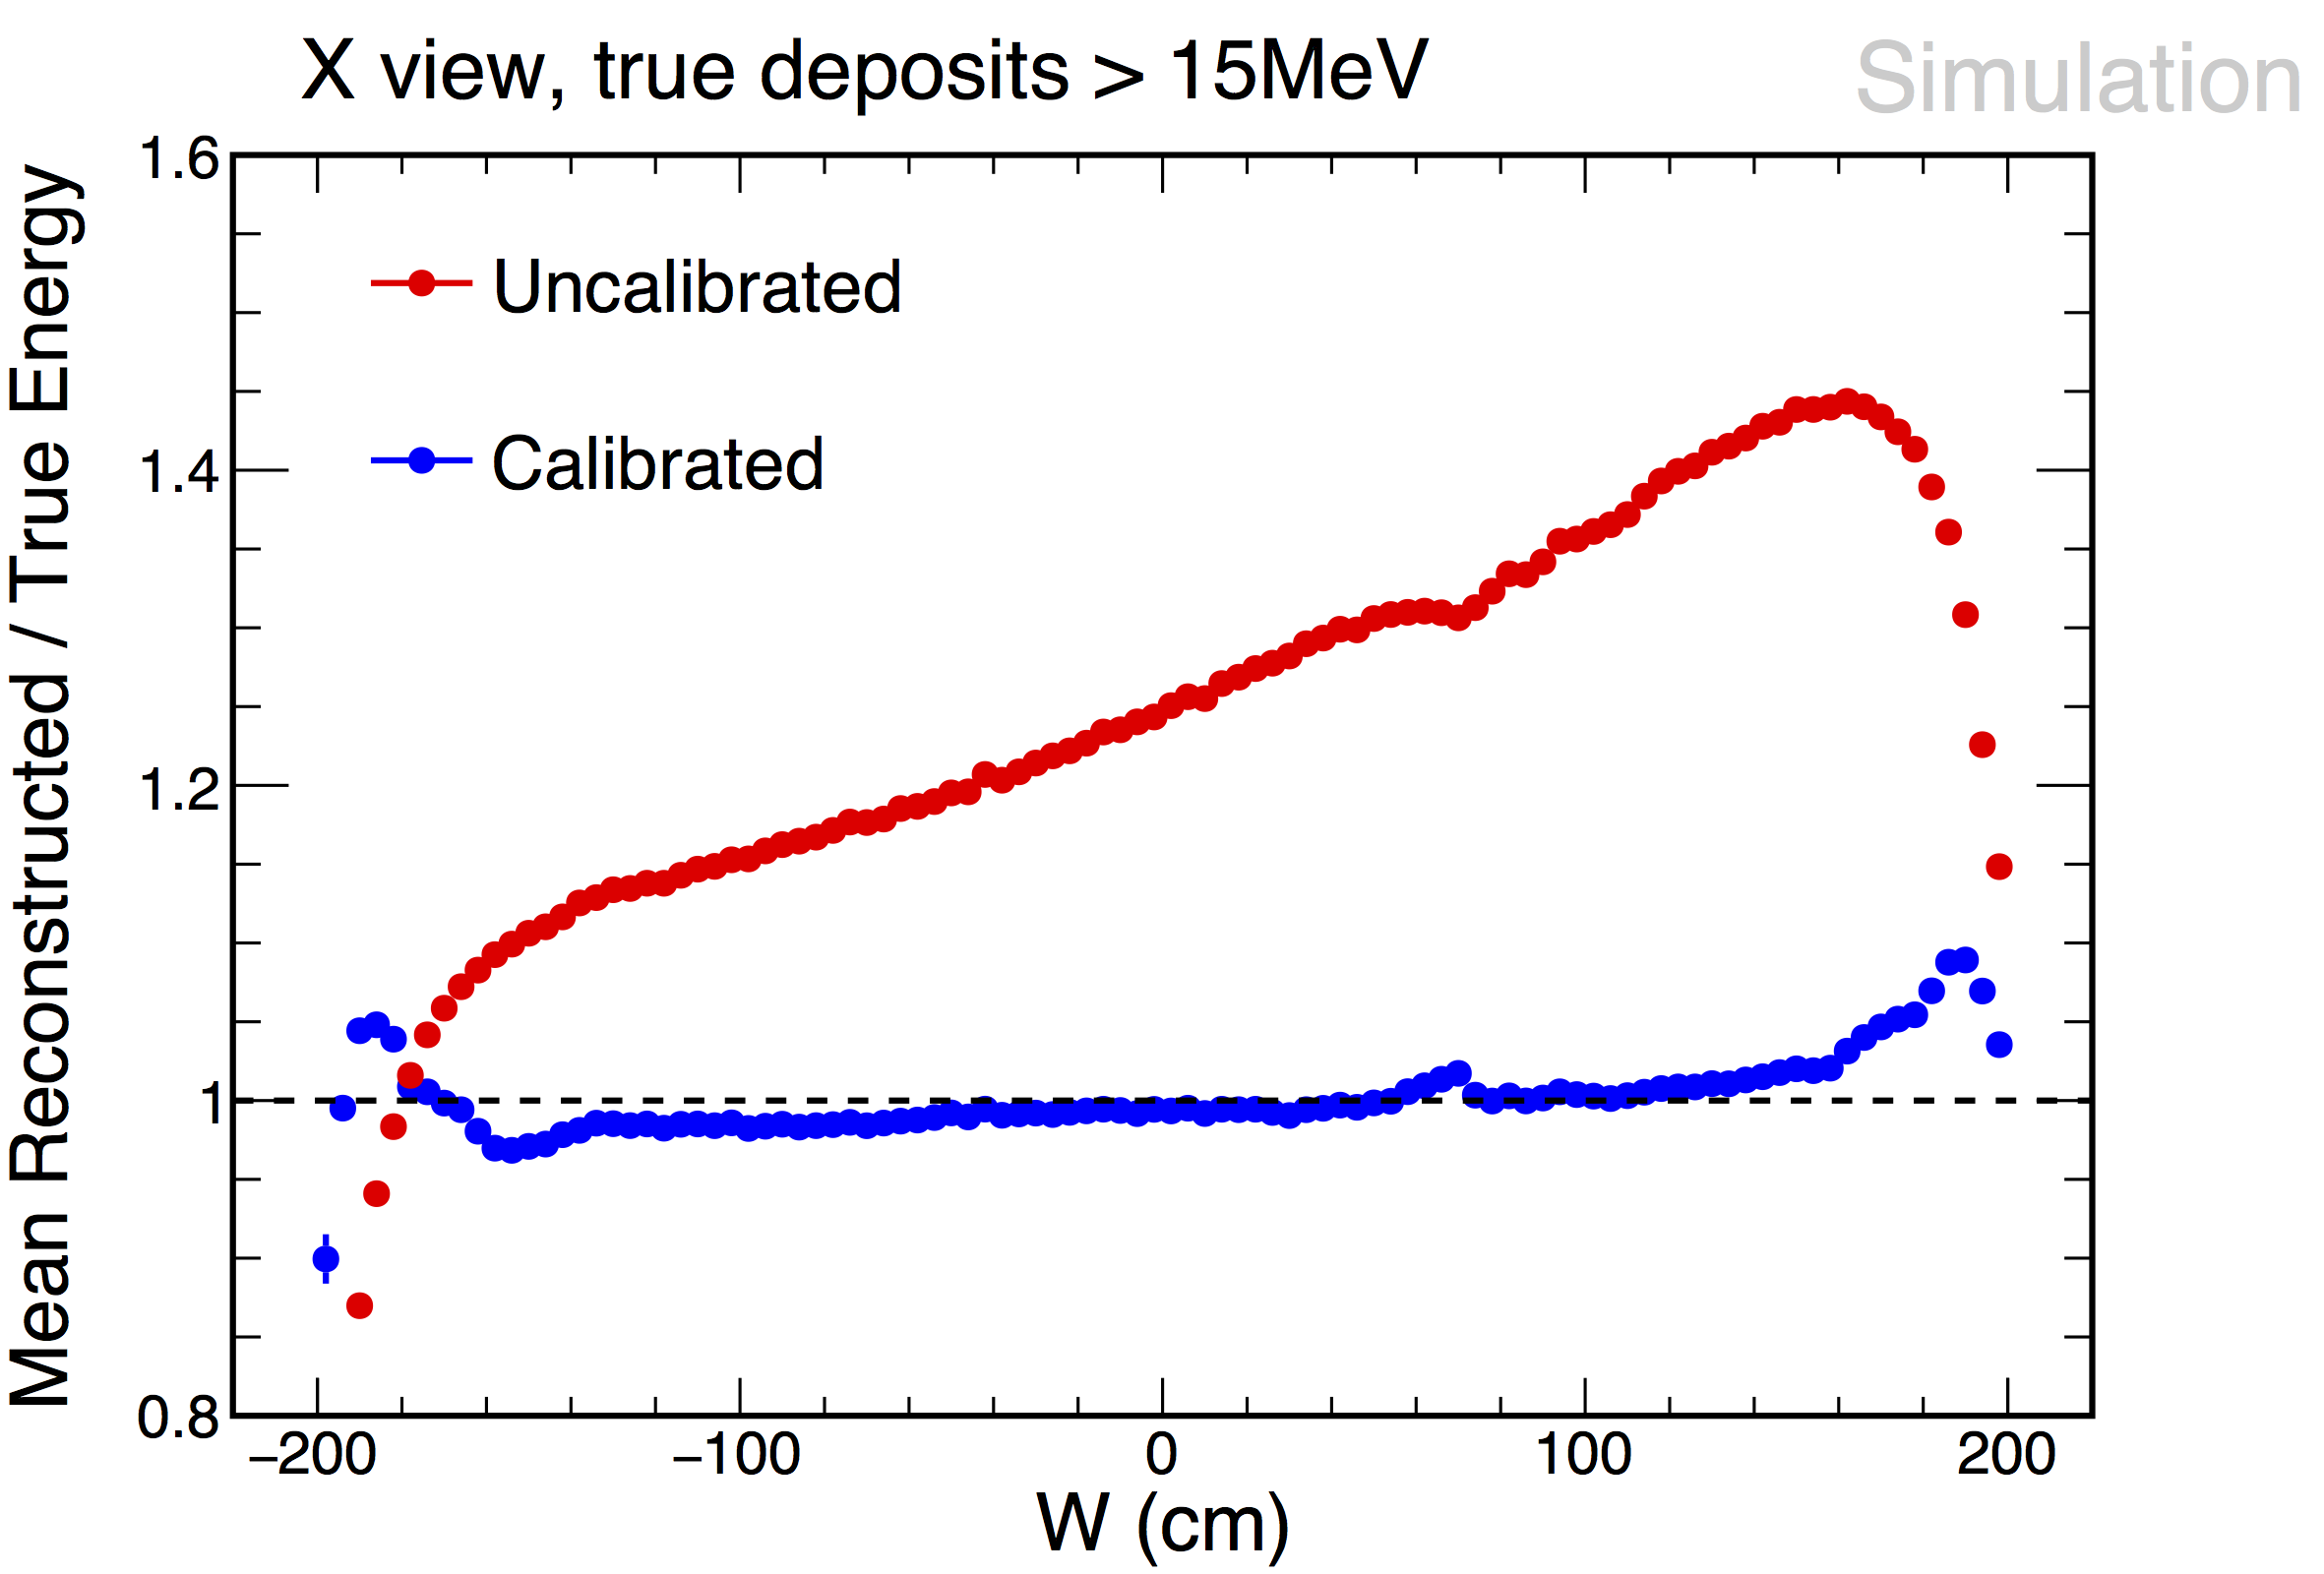
\includegraphics[width=.47\textwidth]{figures/Calib/RelativeNDX.png} &
    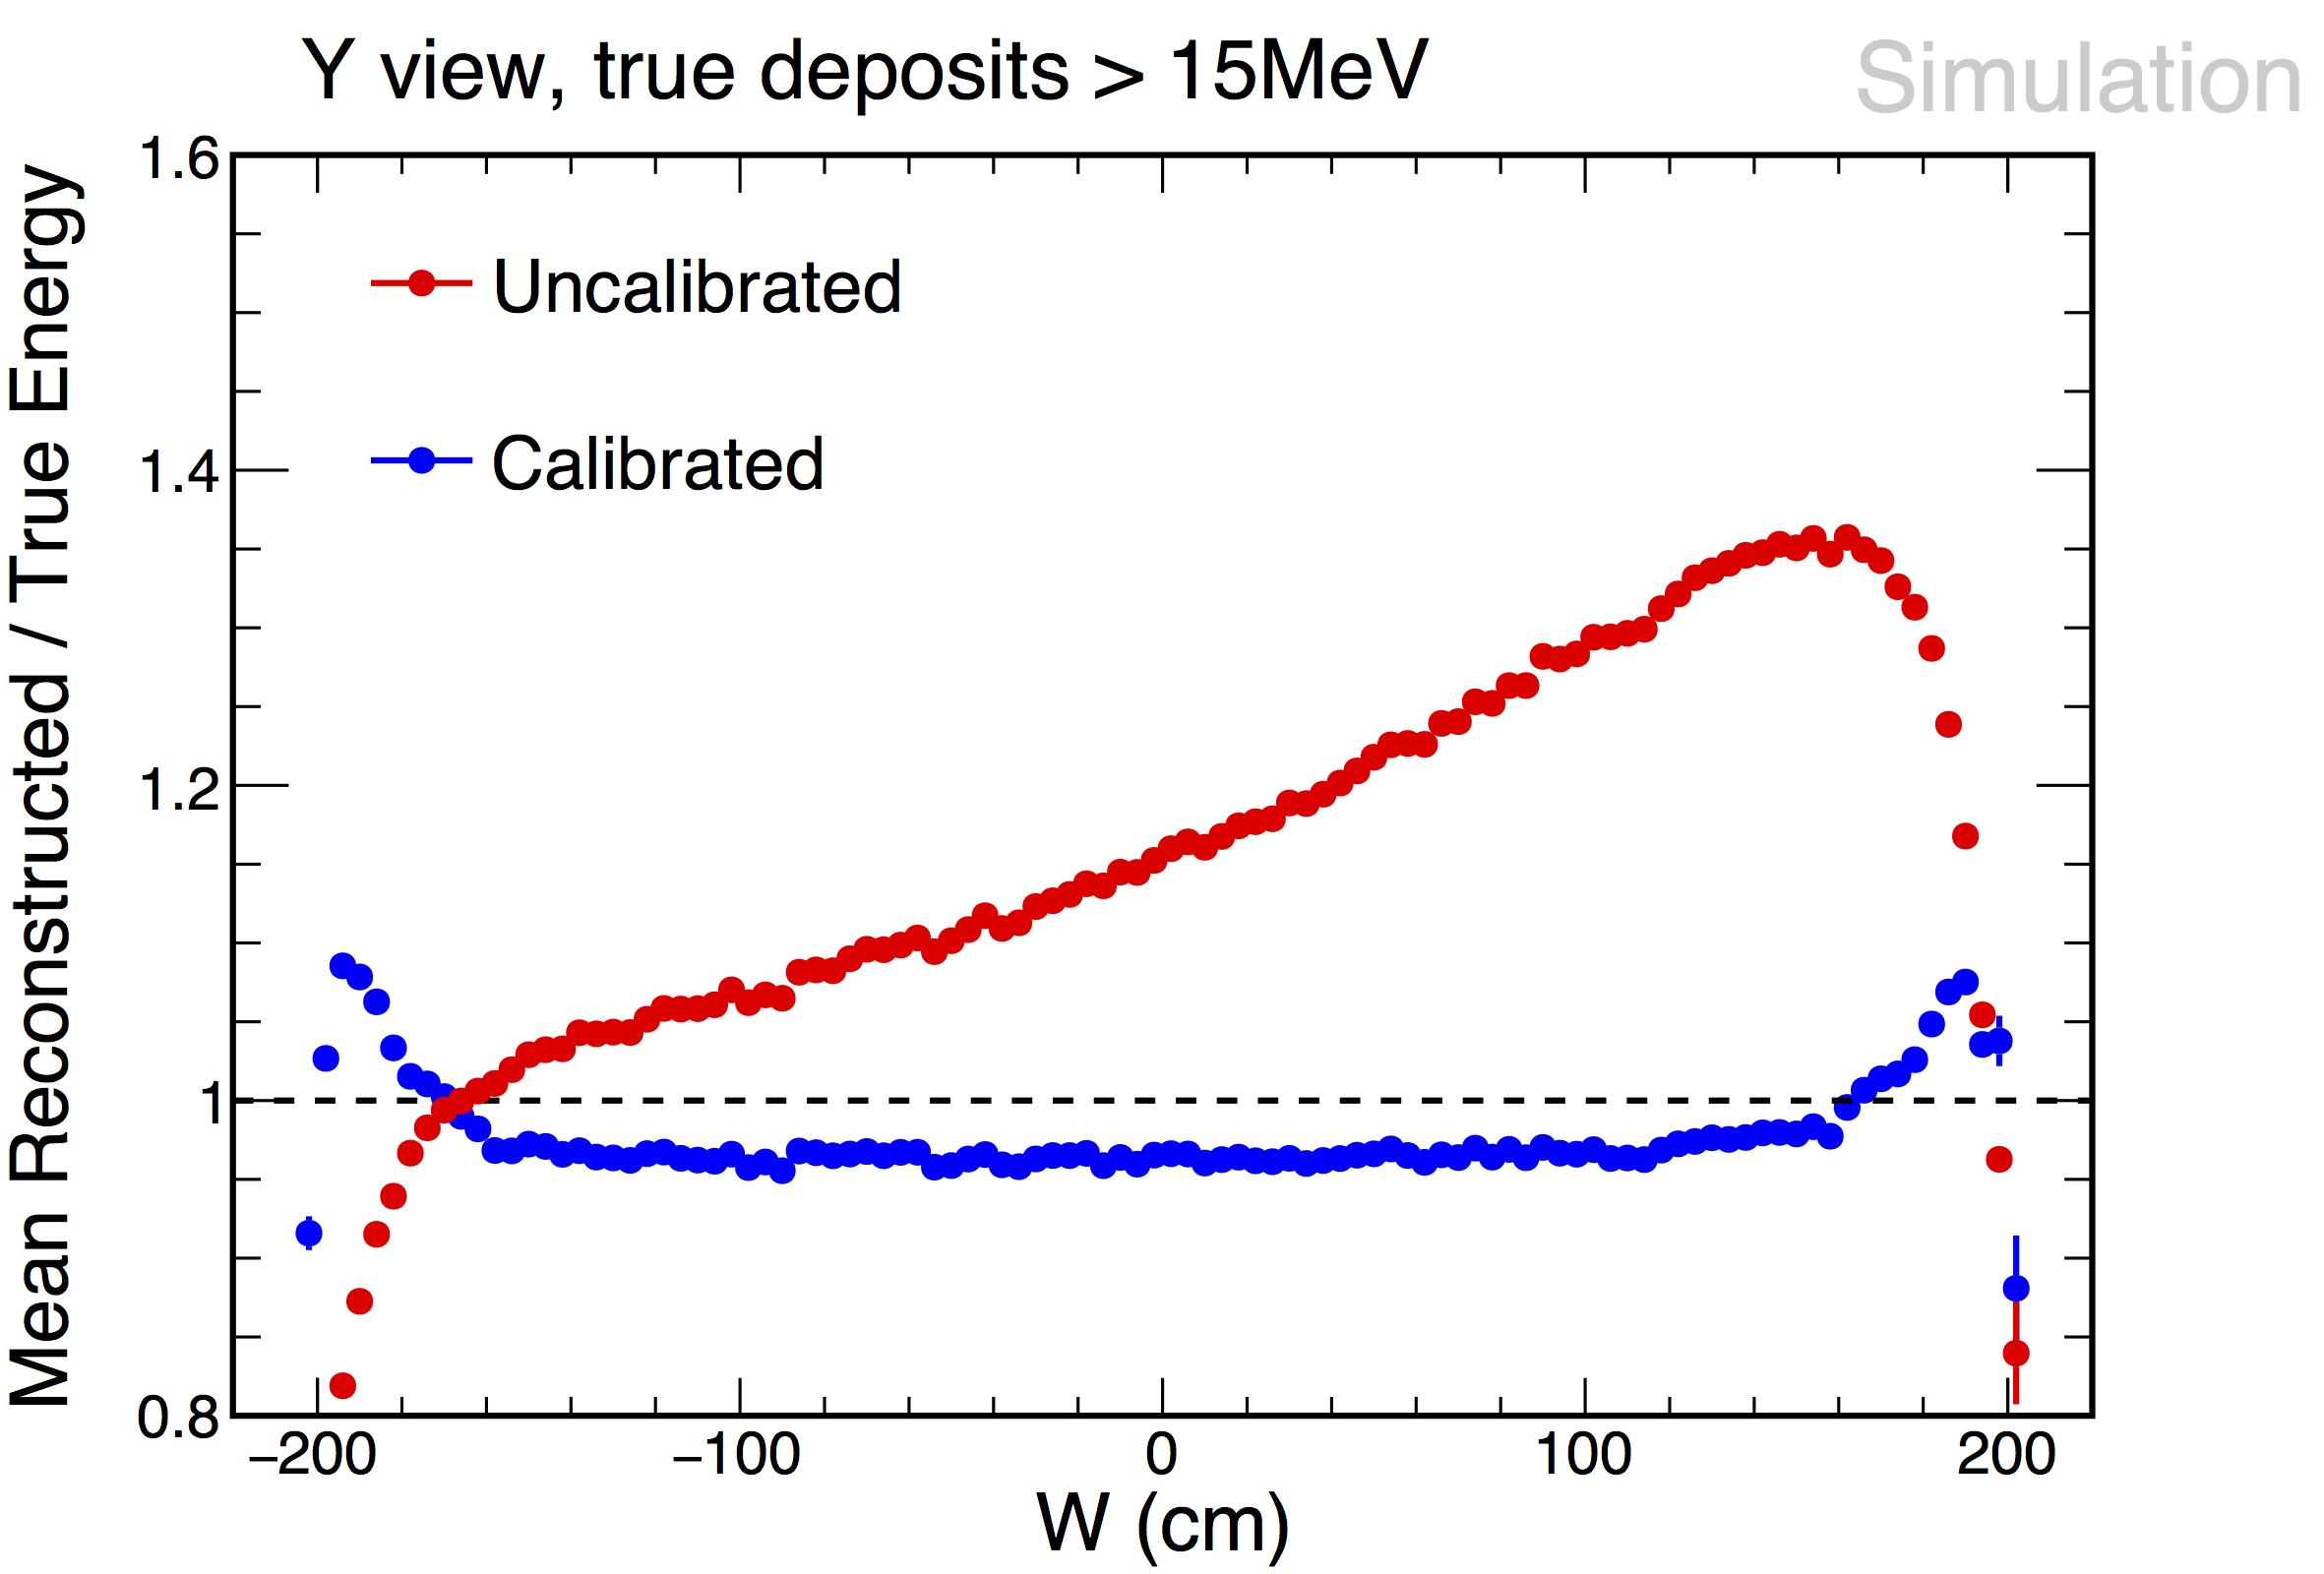
\includegraphics[width=.47\textwidth]{figures/Calib/RelativeNDY.png} \\
    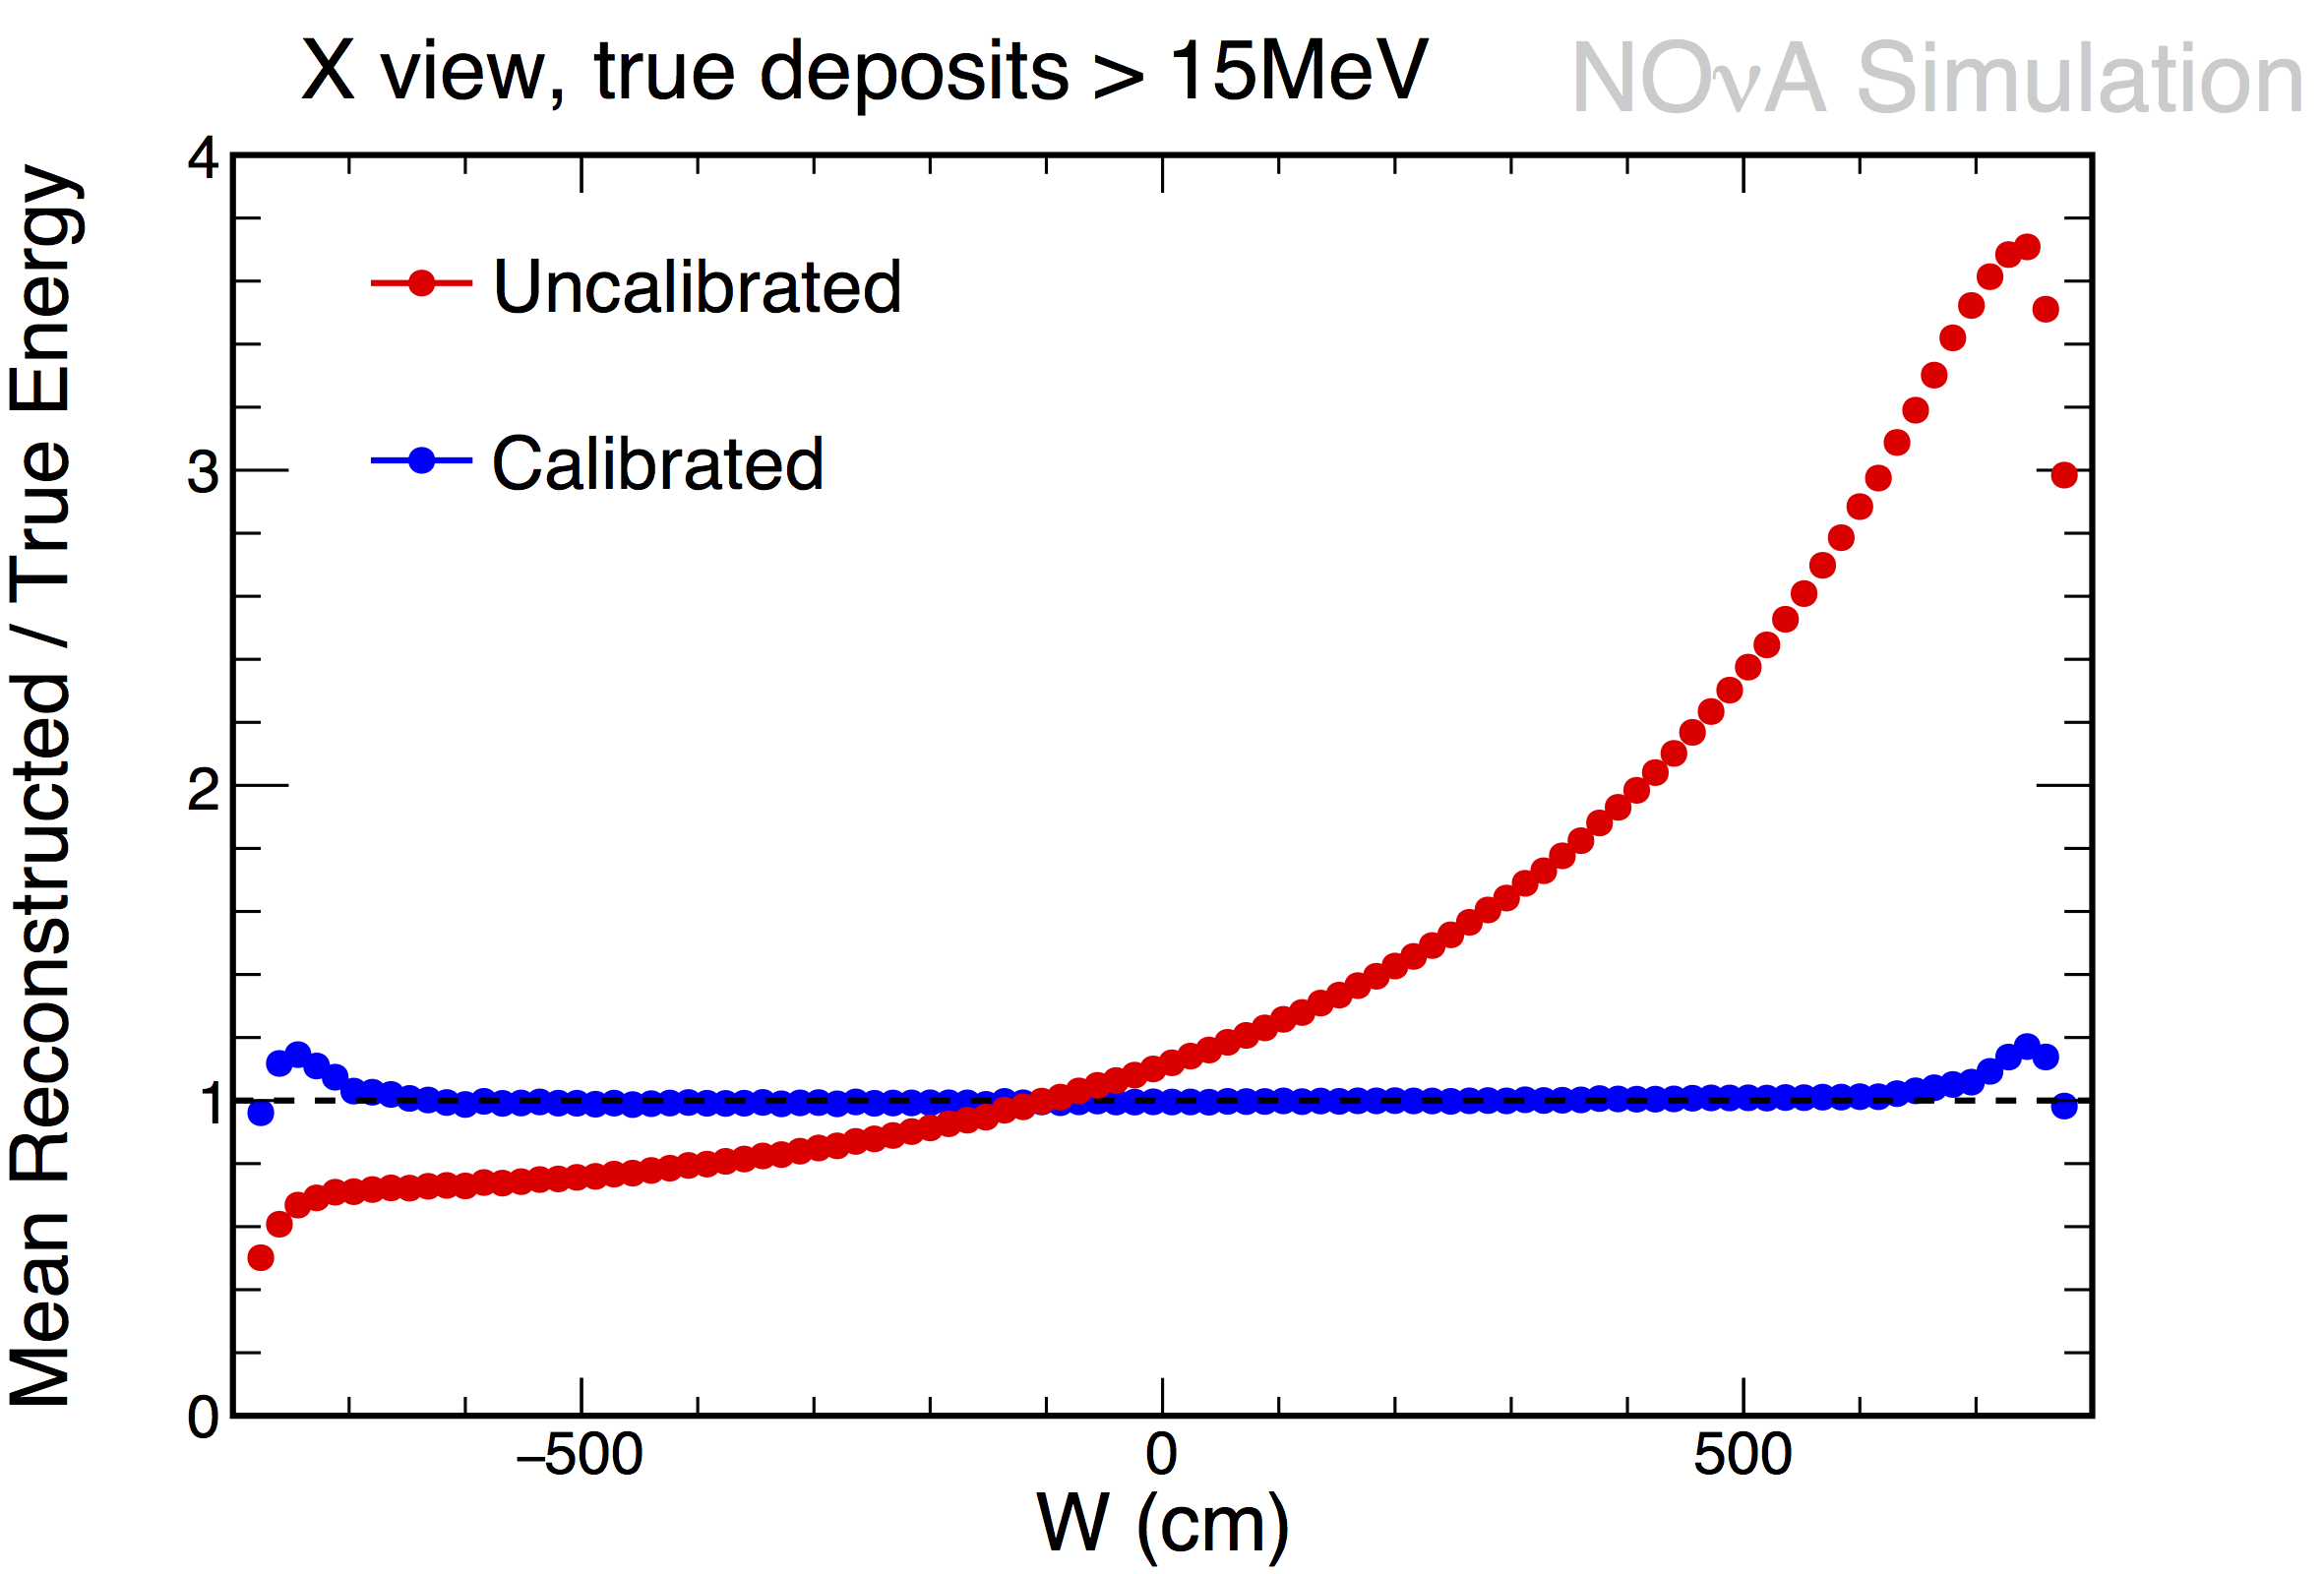
\includegraphics[width=.47\textwidth]{figures/Calib/RelativeFDX.png} &
    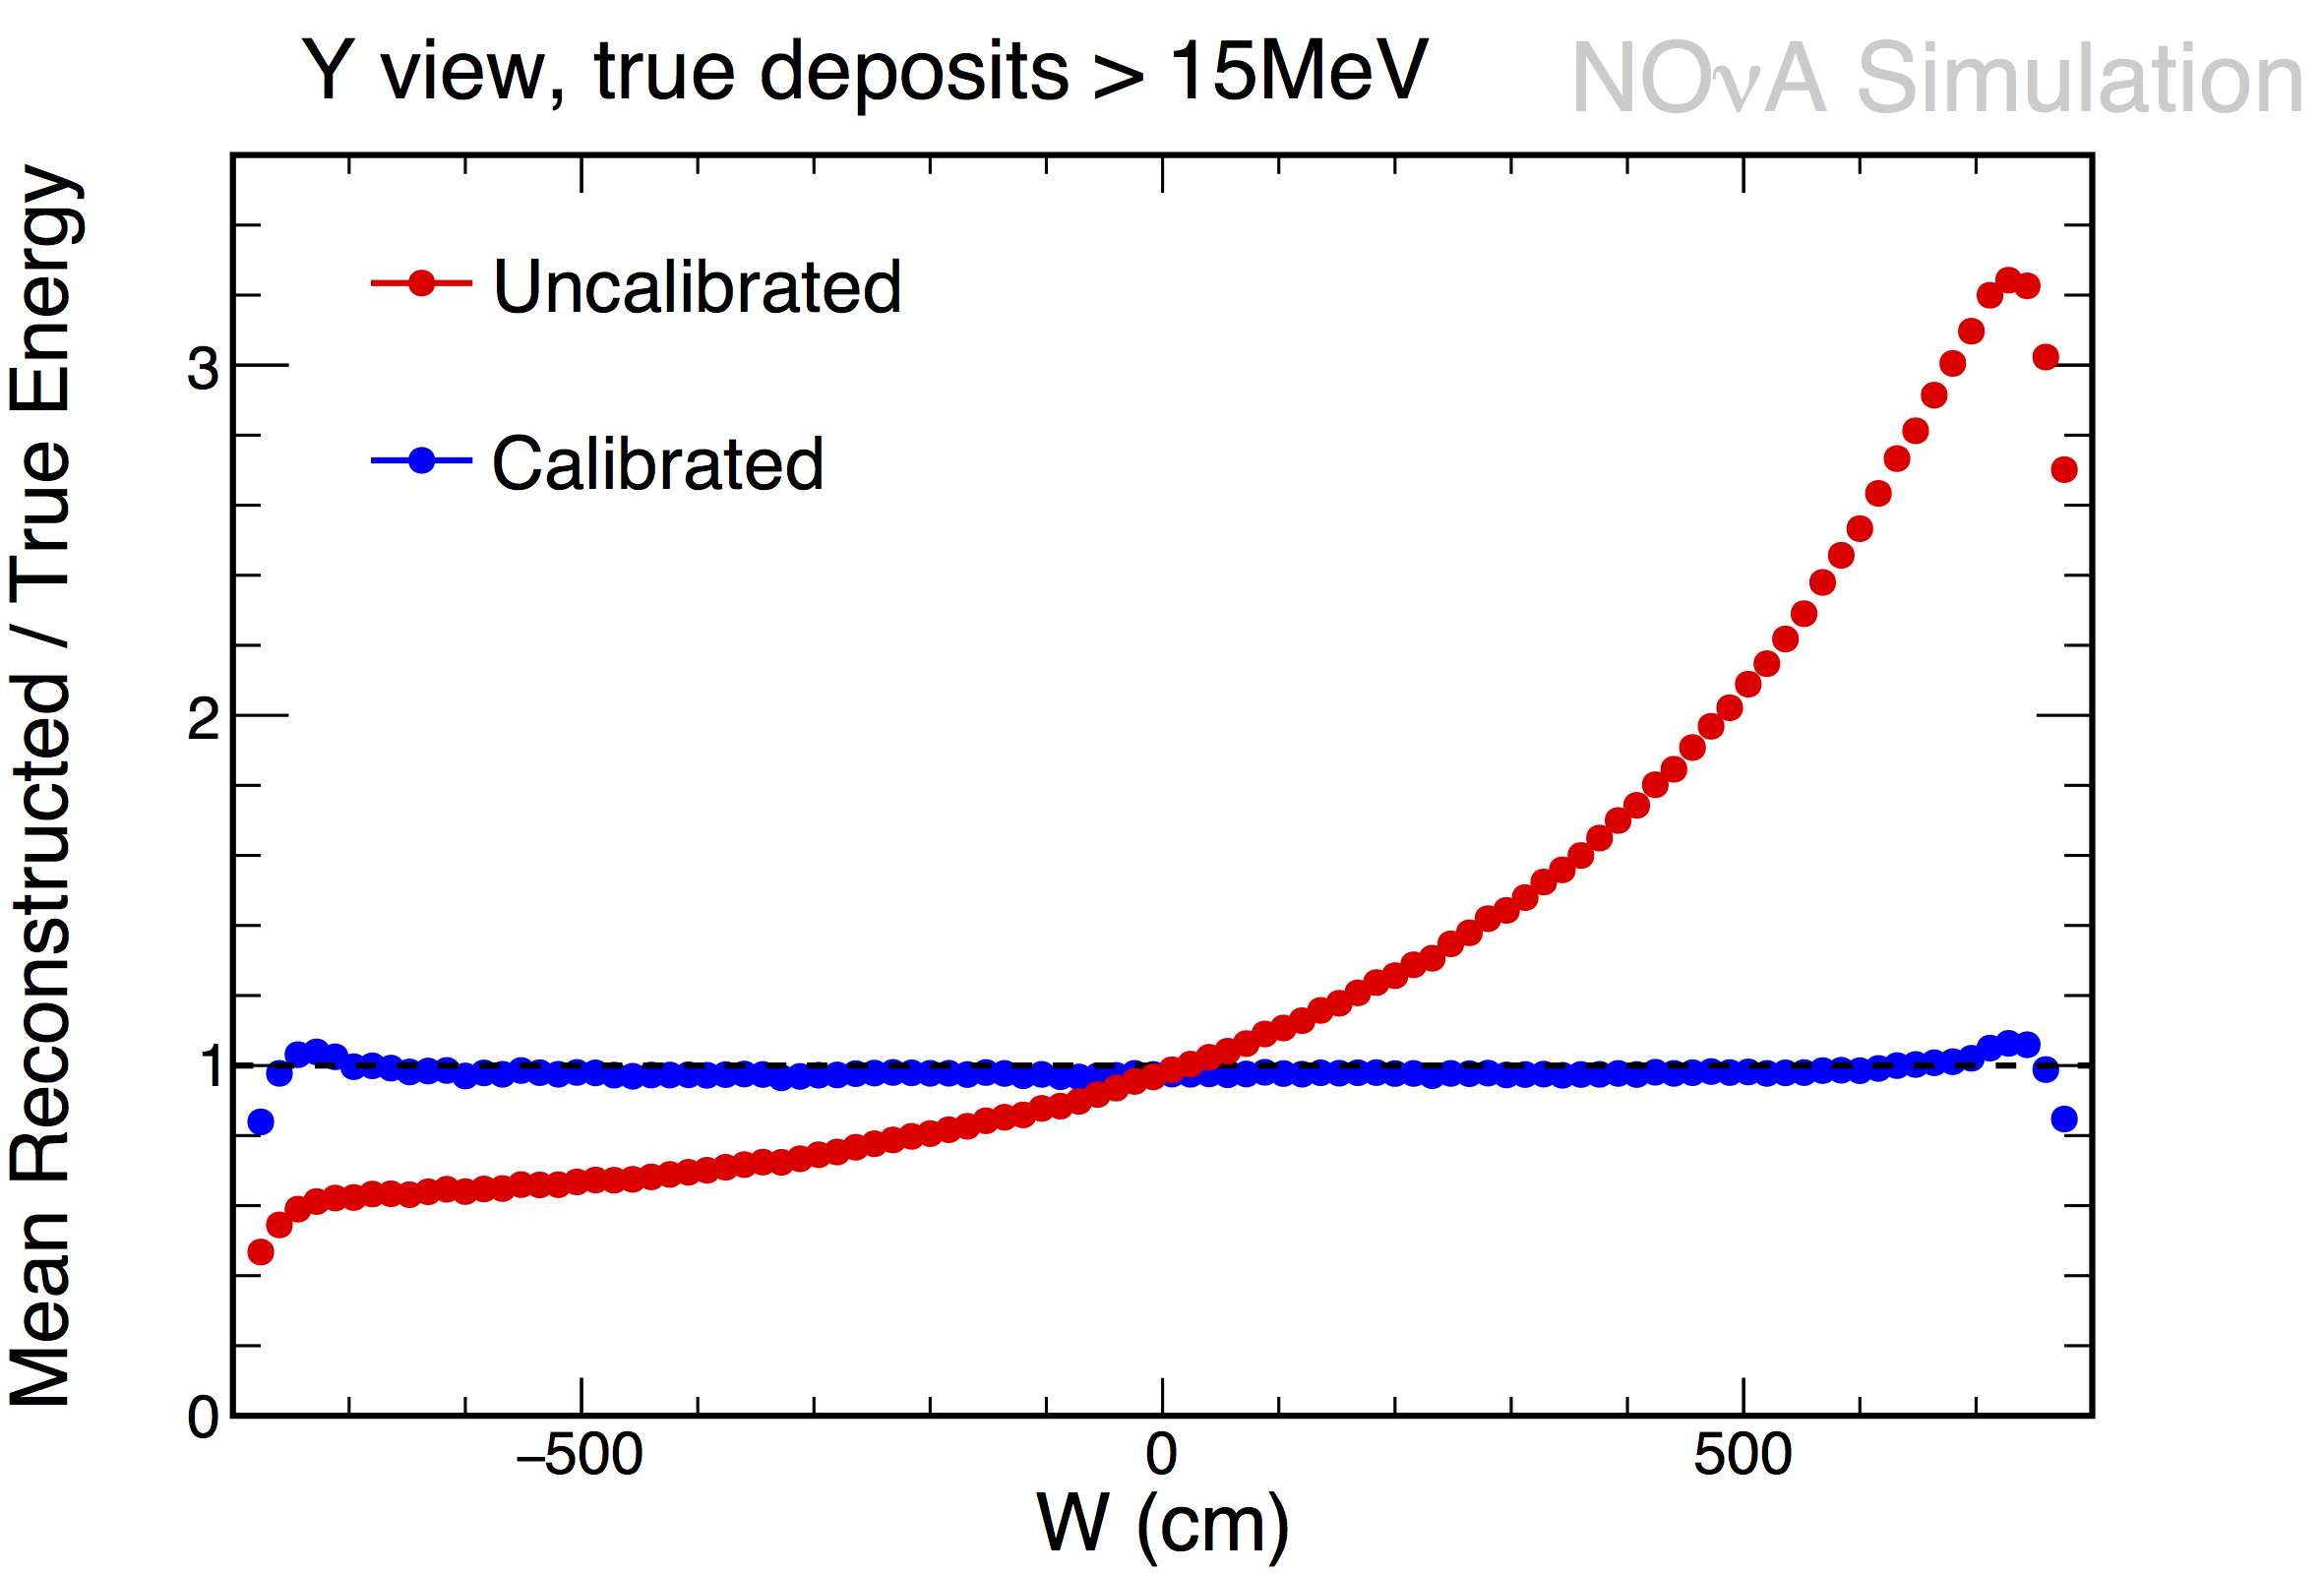
\includegraphics[width=.47\textwidth]{figures/Calib/RelativeFDY.png} \\
  \end{tabular}
  \caption[Relative Calibration Results]{Ratios of mean reconstructed to true energy as a function of distance to readout to assess the performance of the relative calibration. The red points show the ratios before calibration; the blue points after. The left column shows calibration of the X view cells, the right column shows the Y view cells, the top row shows the ND relative calibration results, and the bottom shows the FD results.}
  \label{fig:CalibRelative}
\end{figure}

The absolute calibration is performed after the relative calibration to convert the corrected PE signal into an energy value. Much like the relative calibration, the absolute calibration uses a sample of tricell hits from cosmic ray muons. However, in this case the energy deposited in the cell must be known in order to convert the PE signal into an energy. The energy is known either from external sources \cite{ref:MuonTables} or the Bethe-Block equation \cite{ref:PDG},
\beq
\left\langle-\frac{dE}{dx} \right\rangle = Kz^2 \frac{Z}{A} \frac{1}{\beta^2} \left[ \frac{1}{2} \ln \frac{2 m_e c^2 \beta^2 \gamma^2 W_{max}}{I^2} - \beta^2 - \frac{\delta(\beta\gamma)}{2} \right],
\label{eq:BetheBlock}
\eeq

\n where $K \equiv 4\pi N_A r^2_e m_e c^2$, $r_e$ is the classical electron radius, $m_e c^2$ is the electron rest energy, $z$ is the charge number of the incident particle, $Z$ and $A$ are the atomic number and mass of the stopping material, $\beta$ and $\gamma$ are calculated for the incident particle, $W_{max}$ is the maximum energy transfer to an electron in a single collision, $I$ is the mean excitation energy of electrons in the stopping material, and $\delta(\beta\gamma)$ is the density effect correction to ionization energy loss in the stopping material. With known energy deposition and number of PEs, determining the calibration energy scale is a simple procedure.

The particular energy used for the absolute calibration is the minimum energy deposition of muons through liquid scintillator. For \nova, the liquid scintillator is well approximated as chains of polyethylene, or (C\textsubscript{2}H\textsubscript{4})\textsubscript{n}, for which muons have a minimum average energy loss of $2.079\unit{MeV}$ cm\textsuperscript{2}/g \cite{ref:MuonTables}. The density of the scintillator was measured to be $0.8617\unit{g/cm\textsuperscript{3}}$ \cite{ref:DensityScint}, giving an average energy loss per unit length of $1.792\unit{MeV/cm}$. From simulation, it was determined that this minimum energy deposition occurs between $100 - 200\unit{cm}$ from the end of a muon track, with only a $1.8\%$ variation throughout that region. Figure \ref{fig:CalibAbsDists} shows the distributions of the relative calibration corrected response as a function of distance from the muon track end for FD data and MC and the true energy deposition for the MC.
\begin{figure}[htb]
  \centering
  \begin{tabular}{c c}
    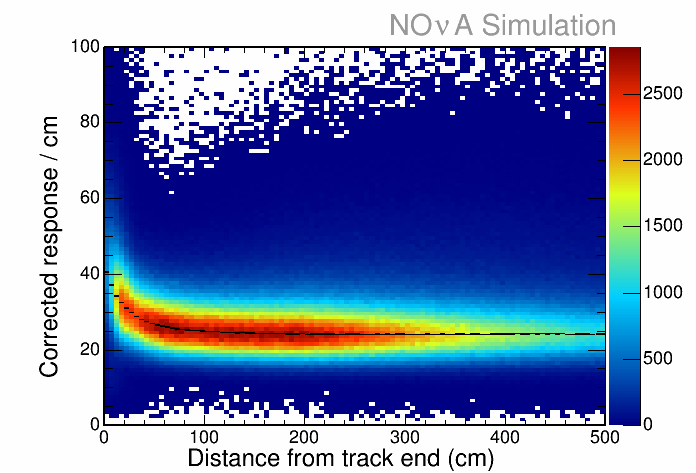
\includegraphics[width=.47\textwidth]{figures/Calib/AbsFDMCPECorrcm.png} &
    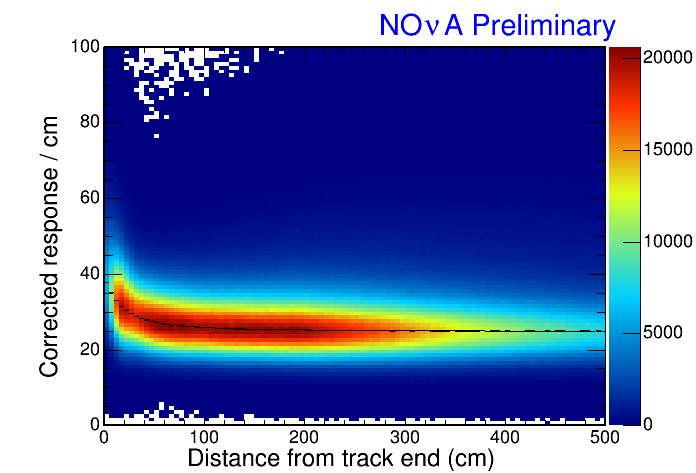
\includegraphics[width=.47\textwidth]{figures/Calib/AbsFDDataPECorrcm.png} \\
    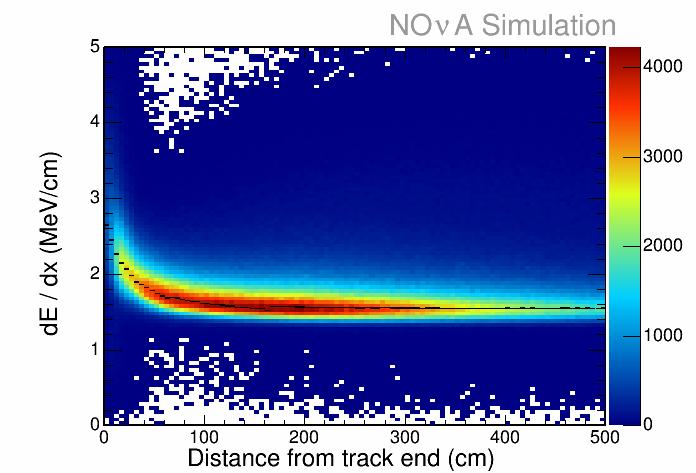
\includegraphics[width=.47\textwidth]{figures/Calib/AbsFDMCdEdx.png} & \\
  \end{tabular}
  \caption[Detector Response to Stopping Cosmic Muons vs Distance to Track End]{Distribution of tricell hits from cosmic ray muon tracks at the FD as a function of distance to the end of the muon track. The top row shows the response in PECorr for both data and MC. The bottom left plot shows the true energy deposited for the MC.}
  \label{fig:CalibAbsDists}
\end{figure}

The absolute calibration energy scale is determined from distributions of tricell hits from stopping muons that occur between $100$ and $200\unit{cm}$ from the end of the muon track. These hits are used to make one dimensional muon energy unit (MEU) distributions of the relative calibration corrected detector response for data and MC called MEU\textsubscript{reco}, and the true energy deposition for MC called MEU\textsubscript{truth}. The calorimetric energy scale is then taken as the mean of the MEU\textsubscript{truth} distribution over the mean of the MEU\textsubscript{reco} distribution. Figure \ref{fig:CalibAbs} shows the distributions of the corrected detector response before the absolute calibration is applied, and the energy distributions after the absolute calibration is applied.
\begin{figure}[htb]
  \centering
  \begin{tabular}{c c}
    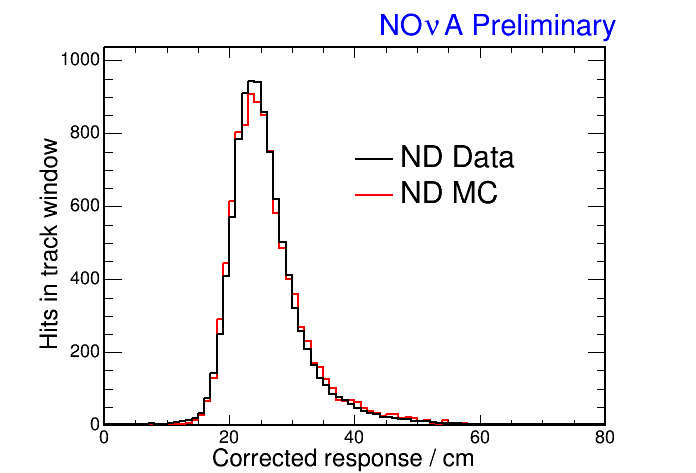
\includegraphics[width=.47\textwidth]{figures/Calib/DataMCNDPECorr.png} &
    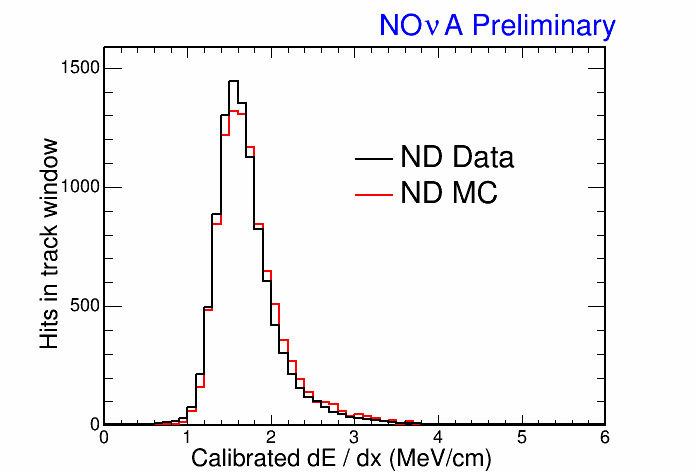
\includegraphics[width=.47\textwidth]{figures/Calib/DataMCNDdEdx.png} \\
    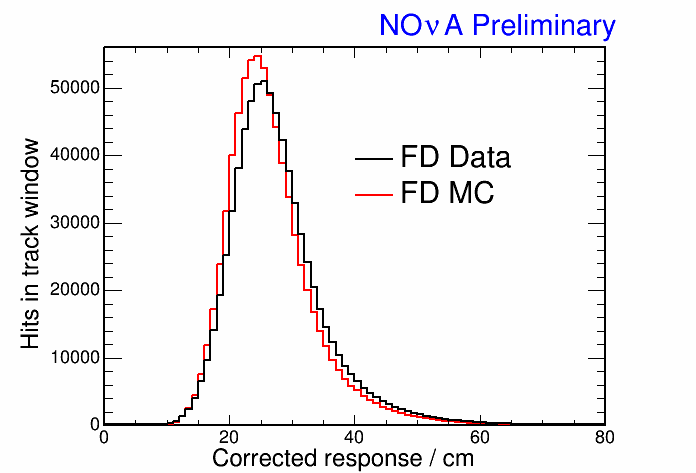
\includegraphics[width=.47\textwidth]{figures/Calib/DataMCFDPECorr.png} &
    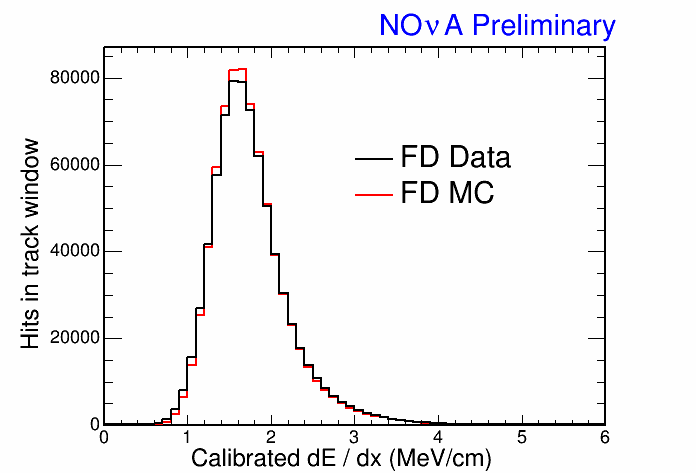
\includegraphics[width=.47\textwidth]{figures/Calib/DataMCFDdEdx.png} \\
  \end{tabular}
  \caption[Absolute Calibration Results]{Distributions of the tricell hits from cosmic ray muons $100-200\unit{cm}$ from the end of the track. The left column shows the relative calibration corrected detector response before the absolute calibration is applied. The right column shows the absolute calibrated energy deposition. The top row shows results for the ND; the bottom shows the FD.}
  \label{fig:CalibAbs}
\end{figure}

At this point the calibration procedure is complete. The calibration constants output by the relative and absolute calibrations are stored in a database so that the raw PE signal in any RawDigit object can be converted into an energy value.

\section{Reconstruction Chain}

The first step in the NC disappearance analysis is the selection of a relatively pure sample of NC events. However, the relatively raw calibrated hits are a far cry from the complete events necessary for the analysis. A set of reconstruction algorithms are thus applied to take individual hits and group them into more complete objects, often providing extra information along the way. The reconstruction procedures begin with the basic grouping of hits in spacetime, and become as complex as applying machine learning algorithms to separate events into different components. The NC disappearance analysis did not have an independent reconstruction chain from the two main \nova~analyses. Rather, the information used for the NC selection discussed in the next chapter was a mixture from the $\nue$ appearance and $\numu$ disappearance analyses. The remainder of this section discusses the reconstruction components relevant to the analysis described in this dissertation.

The first part step in reconstruction is the clustering of hits into separate events, or slices. This is done based on the Density-Based Spatial Clustering of Application with Noise (DBSCAN) algorithm \cite{ref:RecoDBSCAN}. The algorithm as applied to \nova~is described in detail in reference \cite{ref:ThesisMichael}; the main points are summarized here. The DBSCAN algorithm uses a score function to compute a distance between neighboring points. A threshold is set to determine whether two neighbors are close. Points that have more than a set number of neighbors within a that distance are labeled {\em core points}, and the close neighbors of the core points that are not themselves considered core points are labeled {border points}. Clusters are formed by iterating over the hits in an event window, computing whether a point is a core point, then expanding to the neighbors of the core point, and moving to the next cluster when the current one is entirely bounded by border points. At the end of this procedure, slices with more than $3$ hits in each view are made into a `physics' slice, and any hits not assigned to a cluster are placed into a `noise' slice.

The score function used between two hits in the slicing algorithm is
\beq
\epsilon = \left( \frac{ \Delta T - \vert \Delta \vec{r}/c \vert }{ T_{res} } \right)^2 + \left( \frac{ \Delta Z }{ D_{pen} } \right)^2 + \left( \frac{ \Delta XY }{ D_{pen} } \right)^2 + \left( \frac{ PE_{pen} }{ PE } \right)^5,
\label{eq:SlicerScore}
\eeq

\n $T_{res}$ is the timing resolution of the hits added in quadrature, $D_{pen}$ is a distance penalty, $PE$ is the number of photoelectrons in both hits added in quadrature, and $PE_{pen}$ is a penalty on the number of photoelectrons. Hits that are in the same view vs opposite views are handled slightly differently. For hits in the same view, $\Delta \vec{r}$ is calculated in two dimensions. For hits in opposite views, $\Delta \vec{r}$ is one dimensional, $\Delta XY$ is 0, and $D_{pen}$ is replaced with a separate, smaller, opposite view plane penalty. $T_{res}$ was set individually for each hit during the timing calibration, discussed in reference \cite{ref:TNCalib}. The exponent on the PE term was set at $5$ as the PE spectrum for noise falls as $PE^{-2.5}$.

The free parameters and their values are summarized in Table \ref{tab:SlicerParams}. The parameters were tuned and the performance of the algorithm was measured based on two metrics, completeness, the percentage of energy deposited in the scintillator from a physics interaction included in a slice, and purity, the percentage of energy in a slice that came from a single physics interaction. Values were tuned separately for the ND and FD. Notably, $PE_{pen}$ was set to 0 for both detectors, effectively removing this term from the distance calculation.
\begin{table}[htb]
  \begin{center}
    \caption[Slicing Algorithm Free Parameters]{A summary of the free parameters used in the slicing algorithm, and the tuned values used for each detector.}
    \label{tab:SlicerParams}
    \begin{tabular}{c c c}
      \hline\hline
      Parameter & ND & FD \\
      \hline
      $\epsilon$, minimum score required to be considered close neighbors & $5.0$ & $2.0$ \\
      Minimum close neighbors required to be considered core point & $4$ & $4$ \\
      $D_{pen}$, distance penalty & $75.0$ & $100.0$ \\
      Opposite view plane penalty & $8$ & $4$ \\
      $PE_{pen}$, penalty on the PE total & $0$ & $0$ \\
      \hline
    \end{tabular}
  \end{center}
\end{table}